% !TEX program = xelatex

\documentclass[11pt]{article}

\usepackage[review]{acl}

% ── Latin / ACL typography ───────────────────────────────────────────
\usepackage{times}
\usepackage{latexsym}

% ── Unicode / XeLaTeX ────────────────────────────────────────────────
\usepackage{fontspec}

% Explicitly keep the main text in Times.
\setmainfont{TeX Gyre Termes}

% ── Bangla ────────────────────────────────────────────────────────────
\newfontface{\bn}{kalpurush.ttf}[
    Script=Bengali,
    Language=Bengali
]

\newcommand{\bangla}[1]{{\bn #1}}

% ── General packages ─────────────────────────────────────────────────
\usepackage{microtype}
%\usepackage{inconsolata}
\usepackage{graphicx}

\renewcommand{\topfraction}{0.92}
\renewcommand{\bottomfraction}{0.75}
\renewcommand{\textfraction}{0.08}
\renewcommand{\floatpagefraction}{0.75}

\setcounter{topnumber}{3}
\setcounter{bottomnumber}{2}
\setcounter{totalnumber}{4}

\usepackage{booktabs}
\usepackage[table]{xcolor}
\usepackage{multirow}
\usepackage{amsmath}
\usepackage{amssymb}
\usepackage{tabularx}

\usepackage{tikz}
\usetikzlibrary{
    arrows.meta,
    positioning,
    fit,
    backgrounds,
    calc
}

% ── Space discipline ─────────────────────────────────────────────────
\setlength{\abovecaptionskip}{3pt}
\setlength{\belowcaptionskip}{0pt}
\setlength{\textfloatsep}{9pt plus 2pt minus 2pt}
\setlength{\floatsep}{8pt plus 2pt minus 2pt}
\setlength{\intextsep}{8pt plus 2pt minus 2pt}
\setlength{\dbltextfloatsep}{9pt plus 2pt minus 2pt}
\setlength{\dblfloatsep}{8pt plus 2pt minus 2pt}

% ── Theme ────────────────────────────────────────────────────────────
\definecolor{cLaya}{HTML}{27EBF5}
\definecolor{cLod}{HTML}{F127F5}
\definecolor{cJev}{HTML}{F5C827}

\definecolor{fLaya}{HTML}{BEF9FC}
\definecolor{fLod}{HTML}{FCCFFD}
\definecolor{fJev}{HTML}{FCECB3}

\definecolor{fGrey}{HTML}{CCCCCC}
\definecolor{fGreyD}{HTML}{4D4D4D}

\newcommand{\laya}[1]{\cellcolor{fLaya}#1}
\newcommand{\lod}[1]{\cellcolor{fLod}#1}
\newcommand{\jev}[1]{\cellcolor{fJev}#1}
\newcommand{\neu}[1]{\cellcolor{fGrey!55}#1}

\newcommand{\layah}[1]{\cellcolor{cLaya!55}\textbf{#1}}
\newcommand{\lodh}[1]{\cellcolor{cLod!42}\textbf{#1}}
\newcommand{\jevh}[1]{\cellcolor{cJev!62}\textbf{#1}}

% ── Caption swatches ─────────────────────────────────────────────────
\newcommand{\sw}[1]{%
    \textcolor{#1}{\rule[-0.03em]{0.70em}{0.70em}}\,%
}

\newcommand{\swL}{\sw{fLaya}}
\newcommand{\swD}{\sw{fLod}}
\newcommand{\swJ}{\sw{fJev}}
\newcommand{\swG}{\sw{fGrey}}
\newcommand{\swK}{\sw{fGreyD}}

% ── Dataset / intervention macros ────────────────────────────────────
\newcommand{\Drand}{\textsc{d-rand}}
\newcommand{\Dsurf}{\textsc{d-surf}}
\newcommand{\Dsem}{\textsc{d-sem}}
\newcommand{\Dlit}{\textsc{d-lit}}
\newcommand{\Dhard}{\textsc{d-hard}}
\newcommand{\LAR}{\textsc{lar}}


% ── Probability cells ────────────────────────────────────────────────
\newcommand{\pL}[1]{%
    \cellcolor{fLaya}\textbf{#1}%
}

\newcommand{\pJ}[1]{%
    \cellcolor{fJev}\textbf{#1}%
}

% ── Title ─────────────────────────────────────────────────────────────
\title{
    Captured by the Words: Literal Attraction in Typed Decision Models\\
    Tracks the Test Language Rather Than Capability\\
    on Bangla Idioms
}

\author{Anonymous Submission}




\begin{document}
\maketitle

\begin{abstract}
Decision models, non-generative scorers that report a probability over
caller-supplied options and emit no text, are increasingly deployed as routers,
classifiers and guardrails. Because they generate nothing, rationales and
chain-of-thought do not apply, and idioms make token attribution hard to
interpret: for an expression whose figurative reading is not recoverable from its
parts, it is unclear what a per-word contribution would mean. We therefore audit three such models, an encoder scorer, a
decoder scorer and a closed commercial API, entirely through interventions on
the option set, using expert-annotated Bangla idioms that ship with both a gold
figurative gloss and a gold literal gloss. Dropping an idiom's own literal gloss
into the option list captures all three models. Running the full model
$\times$ language matrix over one shared item set shows the failure tracks the
test language rather than capability: every arm is several times more captured in
Bangla than in English on the same paired entries, and the commercial model's
apparent resistance turns out to be a property of the language it was tested in.
Confidence inverts under the same shift, so gating on it does worse than gating
at random, and on a semantics-free option list, where no option carries
information and expected accuracy is $0.25$, the best-calibrated arm still
reports $0.82$ confidence.
Option-order sensitivity, by contrast, separates the two scoring architectures
rather than the three models.
\end{abstract}


% \begin{figure}[t]
% \centering
% 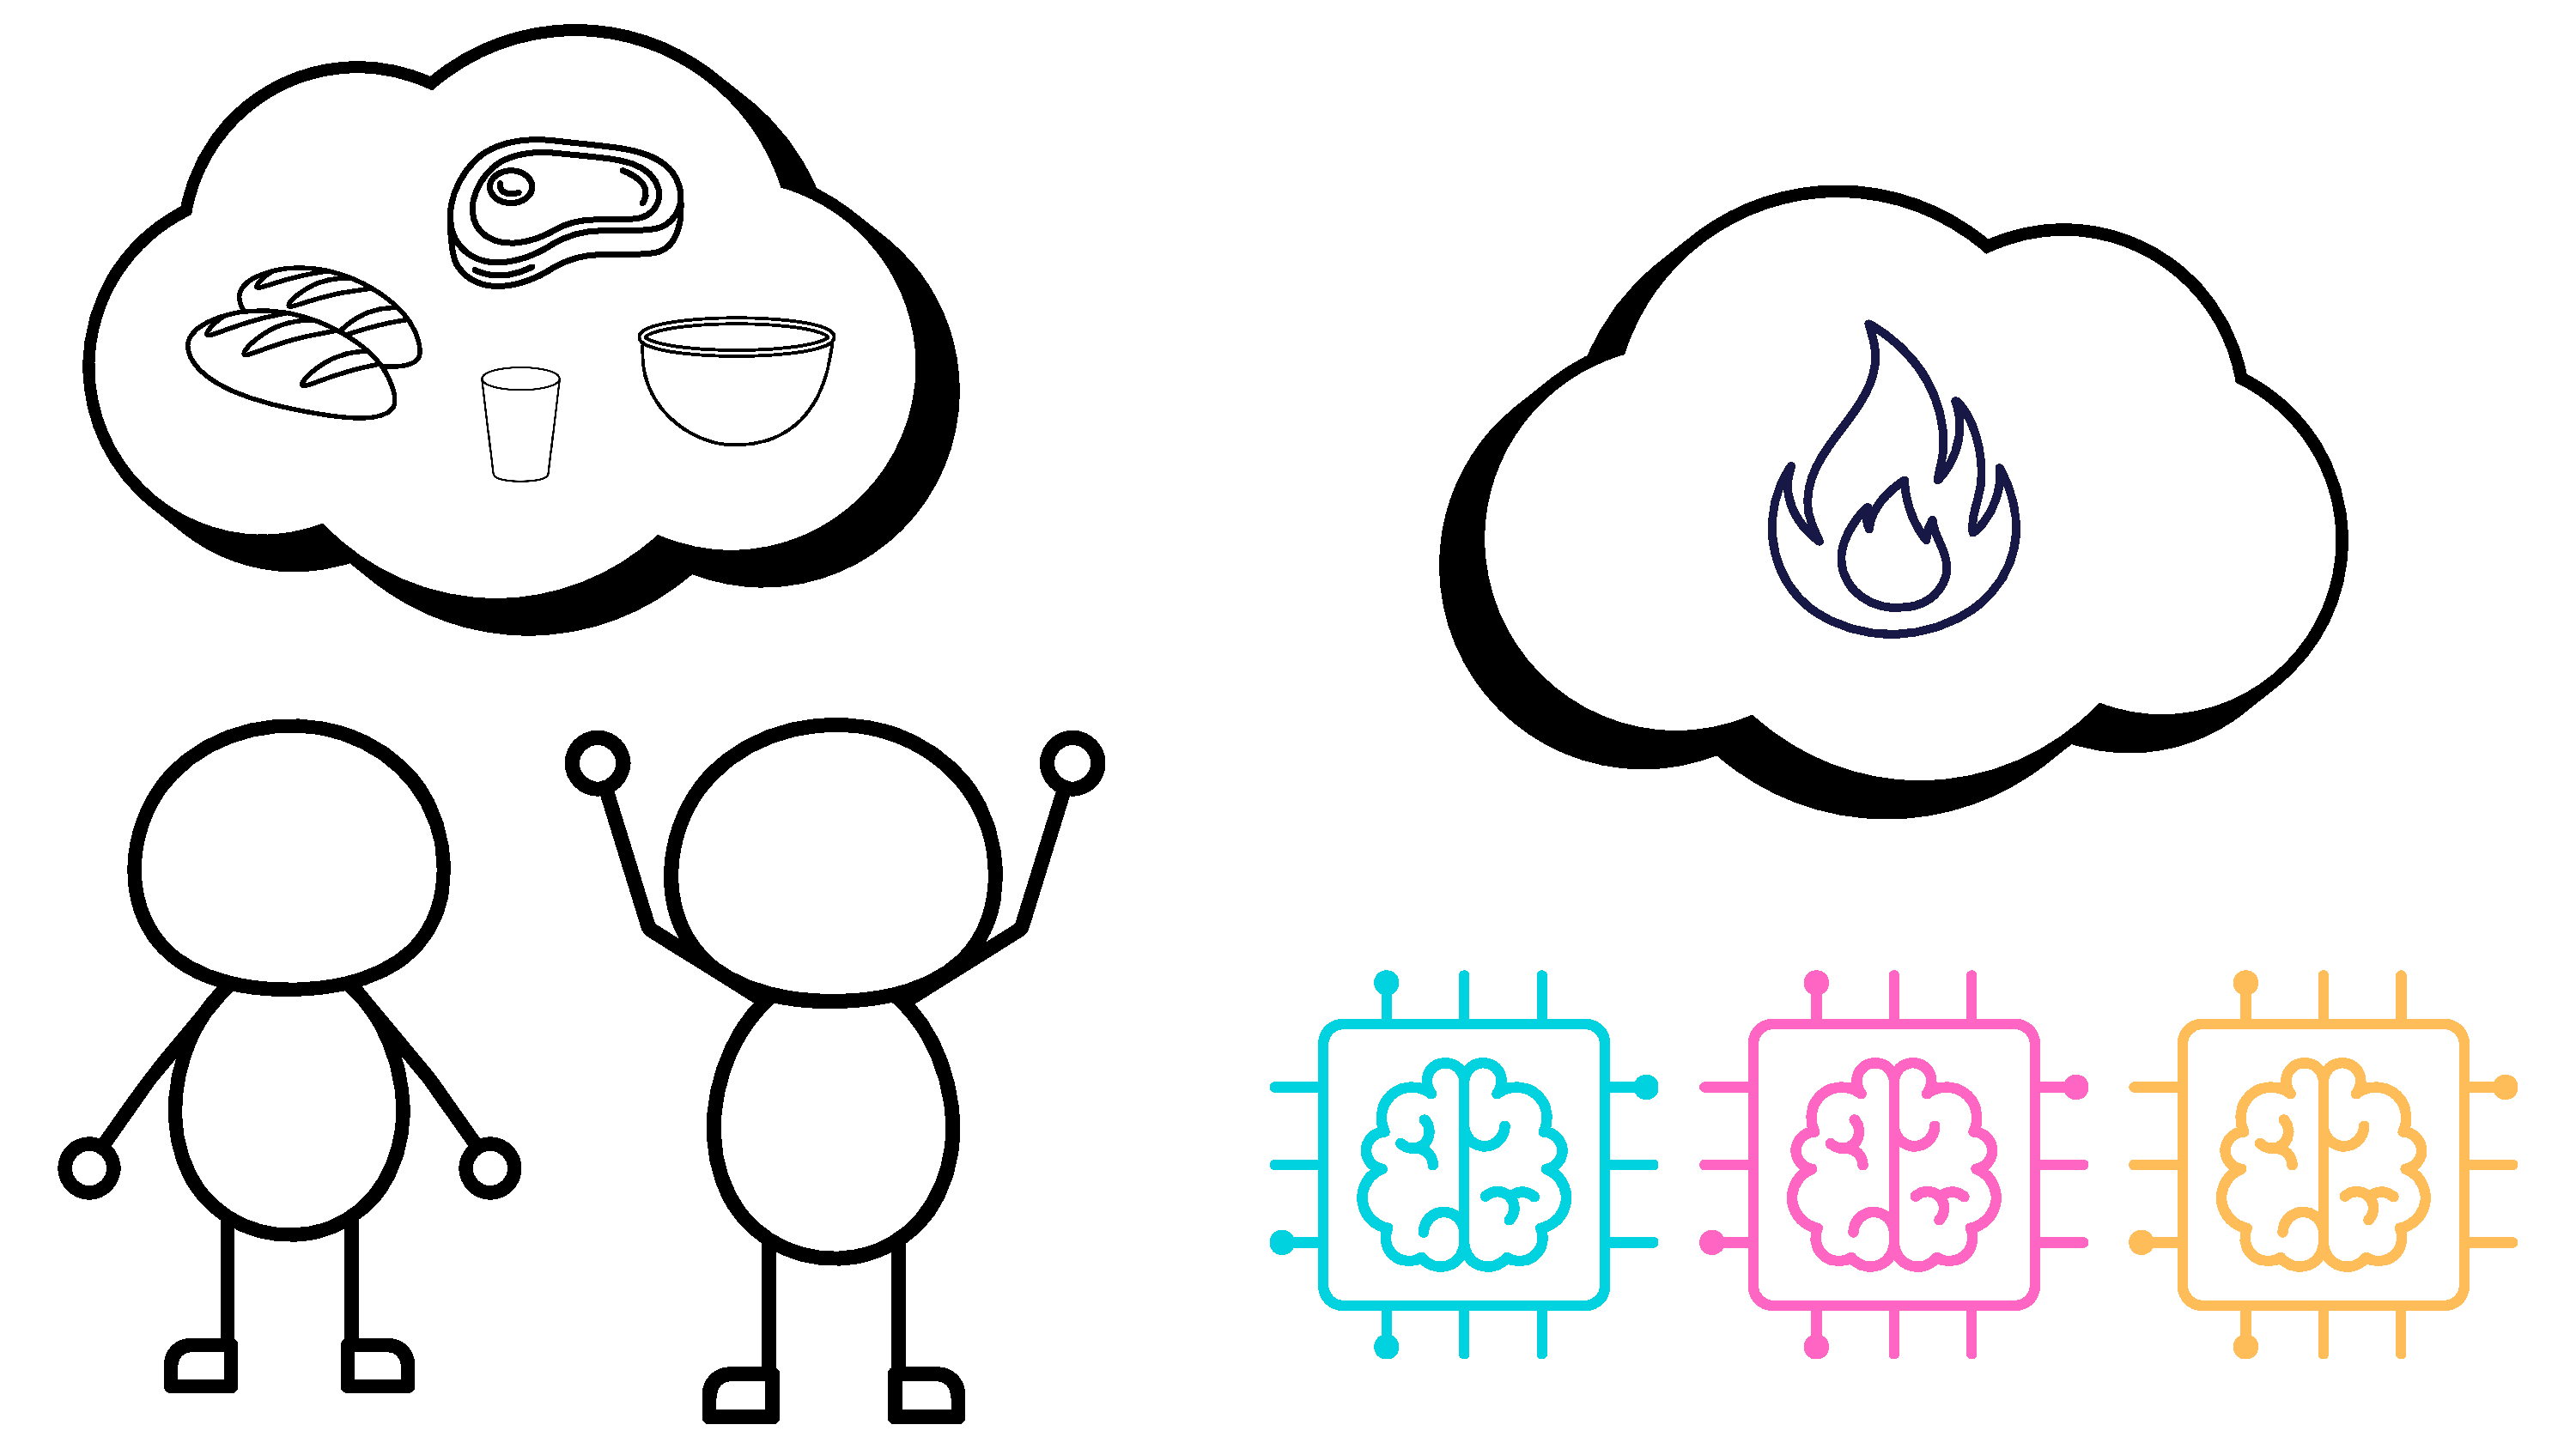
\includegraphics[width=\columnwidth]{figures/fig_bn_teaser_2.pdf}
% \caption{\textbf{The model takes the words.} \emph{Agnibal} is built from the
% words for \emph{fire} and \emph{strength} and means intense hunger; English says
% \emph{fire in the belly}. With both readings in the option list, all three
% models we audit choose the literal one in Bangla, at $p = 1.00$, $0.97$ and
% $0.36$; asked in English with the same four options, two of the three recover.
% Across 3{,}265 items literal attraction falls from $0.731$, $0.918$ and $0.304$
% in Bangla to $0.379$, $0.241$ and $0.047$ in English (\S\ref{sec:capture}).}
% \label{fig:teaser}
% \end{figure}


\begin{figure}[t]
\centering
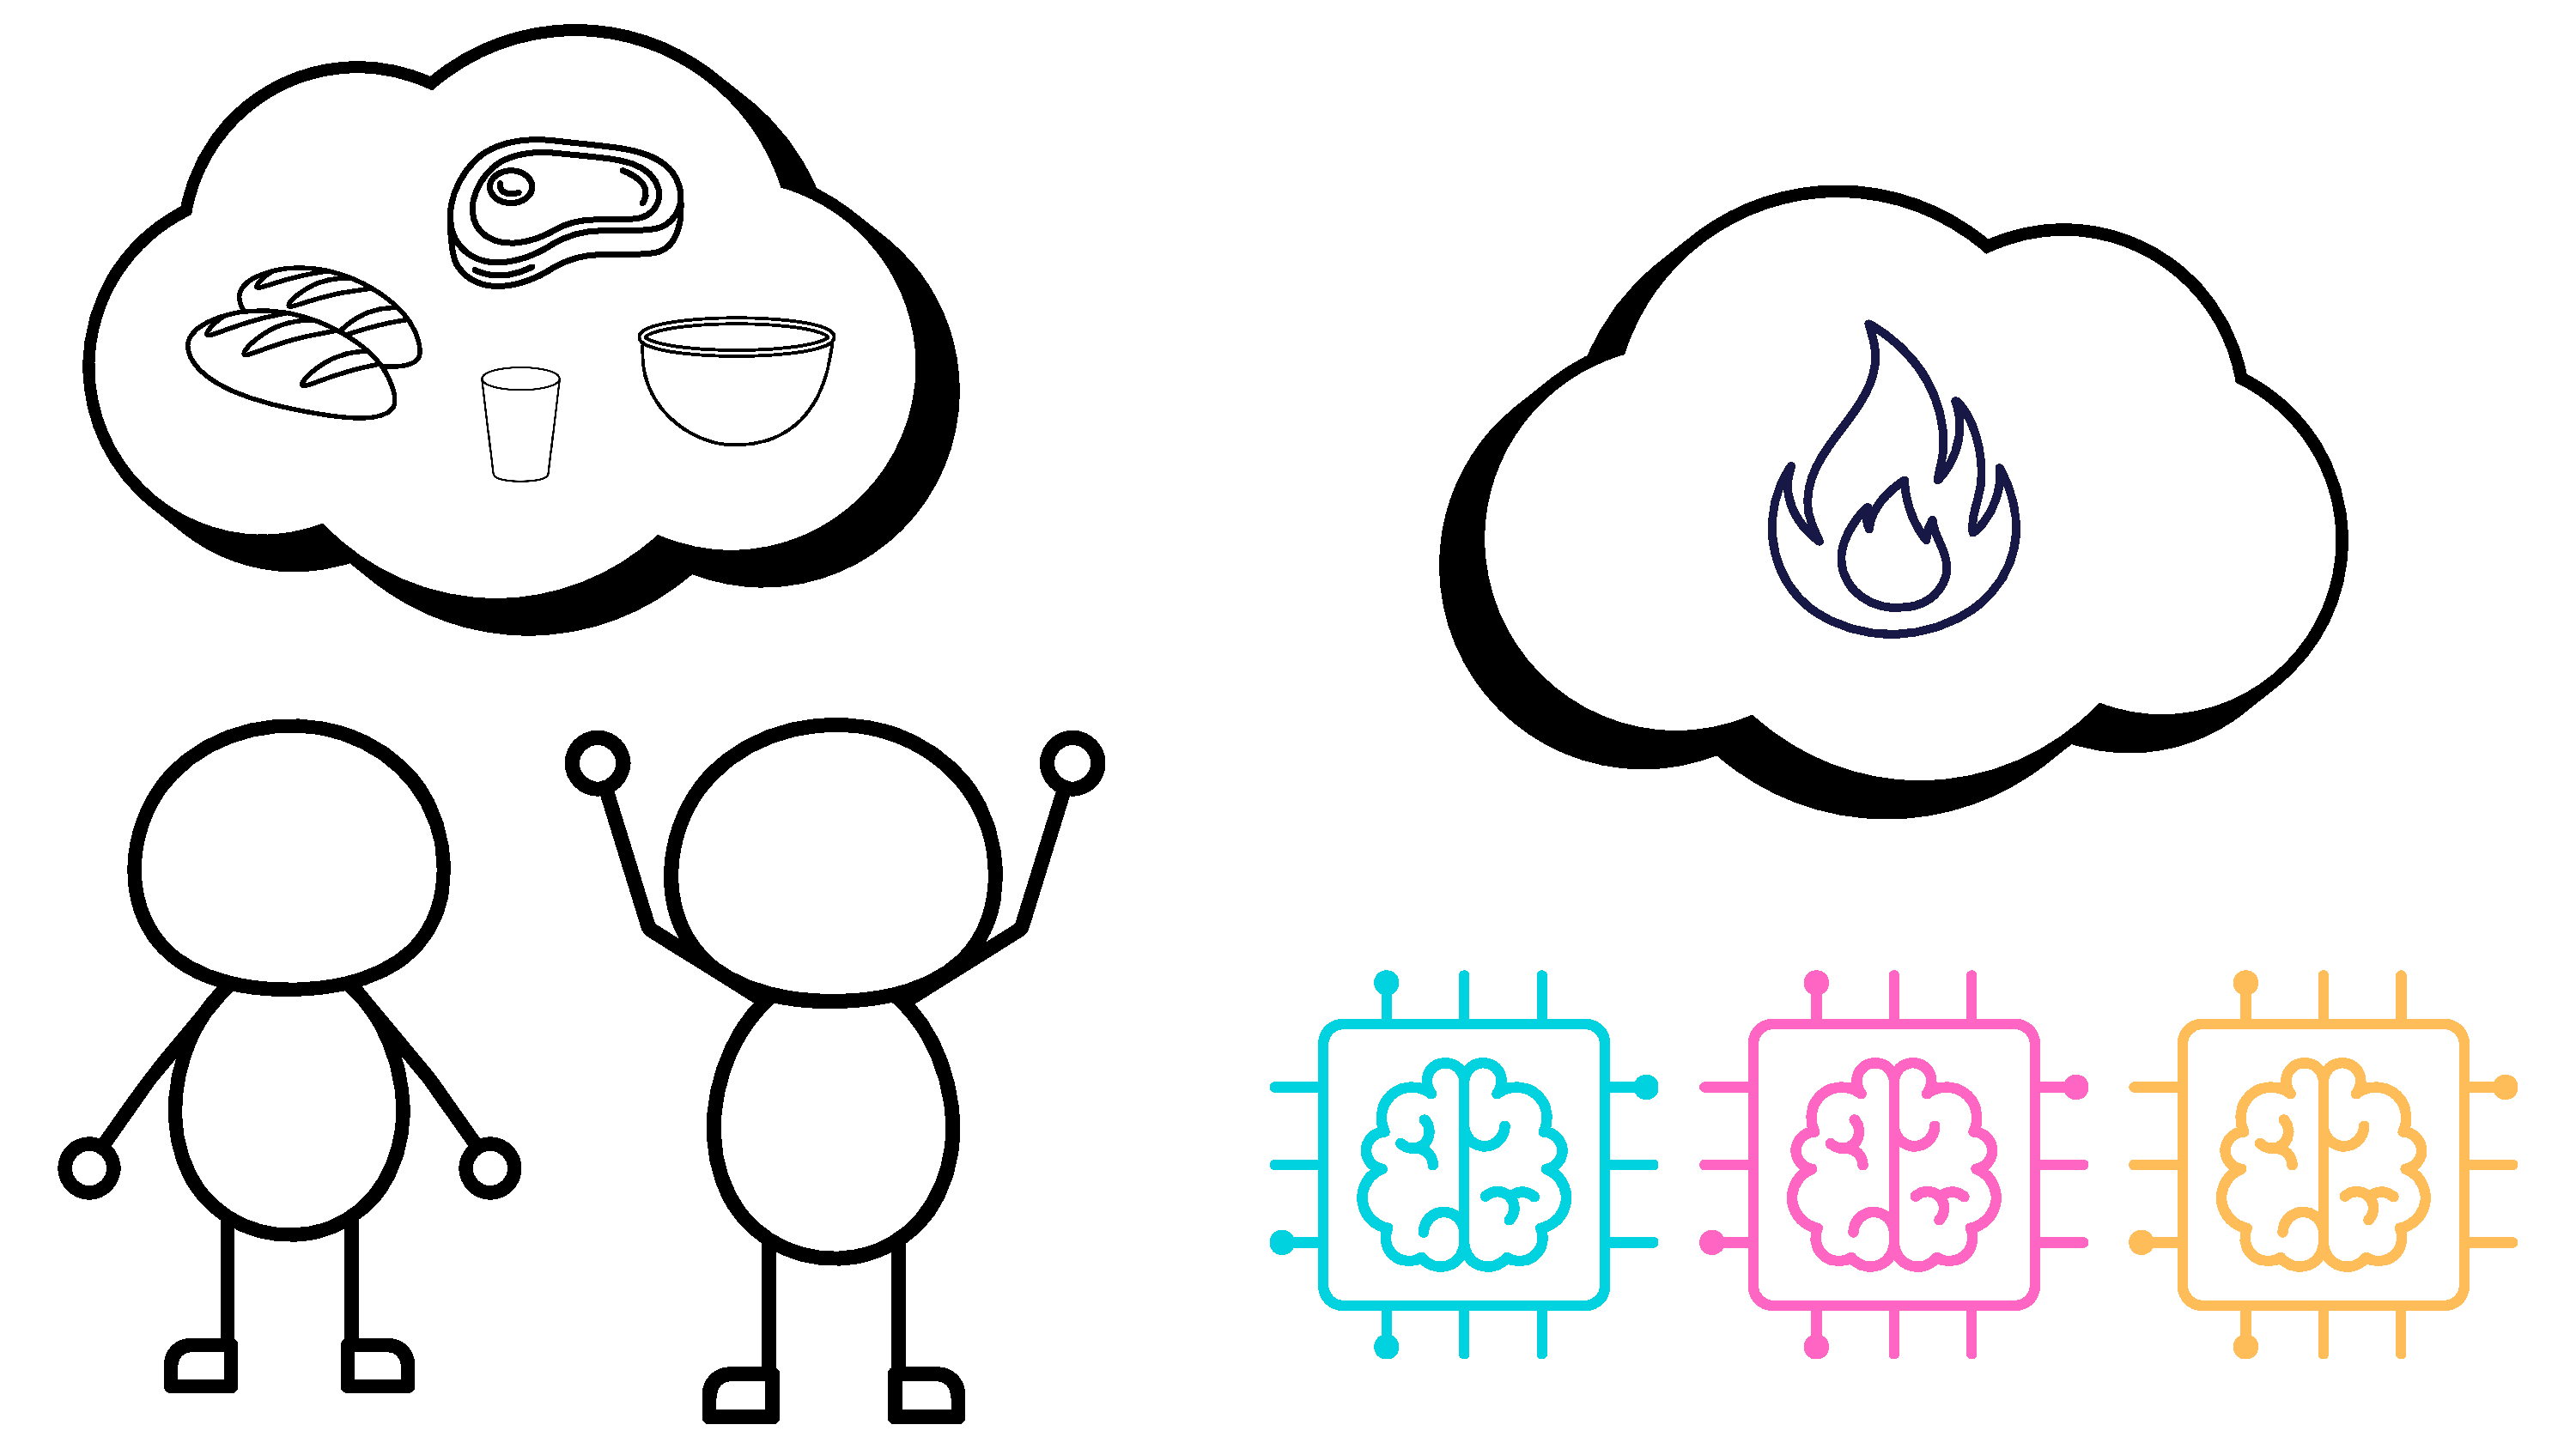
\includegraphics[width=\columnwidth]{figures/fig_bn_teaser_2.pdf}
\caption{\textbf{The model takes the words.}
\textcolor{cyan}{Laya-ml}, \textcolor{magenta}{Lod-lille}, and
\textcolor{orange}{Jev-1.13} are shown in cyan, magenta, and orange,
respectively, throughout the paper. The Bangla idiom
\bangla{অগ্নিবল} (Agnibal) is composed of \bangla{অগ্নি} (\emph{fire}) and
\bangla{বল} (\emph{strength}), but means intense hunger; English
expresses the same concept as \emph{fire in the belly}. When both
readings are placed in the option list, all three models choose the
literal gloss in Bangla, at $p=1.00$, $0.97$, and $0.36$,
respectively; with the same four options in English, two of the three
recover. Across $3{,}265$ paired items, literal attraction falls from
$0.731$, $0.918$, and $0.304$ in Bangla to $0.379$, $0.241$, and
$0.047$ in English (\S\ref{sec:capture}).}
\label{fig:teaser}
\end{figure}

\section{Introduction}

A \emph{decision model} is given a question and a list of candidate options and
returns a probability distribution over exactly those options. It is not
autoregressive, it does not sample, and it produces no text. This class has
grown quickly as infrastructure for routing, intent classification, content
gating and tool selection, precisely because it is cheap, bounded and returns a
number a caller can threshold on. An ecosystem analysis of 2{,}170 public
projects finds it already embedded as a reusable decision component across
domains \citep{ling2026wild}, and proposals now place these models at the
adjudication points of autonomous security harnesses
\citep{santos2026pentest}. The threshold is load-bearing.

That bounded interface is also an explainability problem. There is no rationale
to inspect, no chain of thought to measure for faithfulness
\citep{jacovi2020faithfulness,turpin2023unfaithful}, and in the commercial case
no weights at all. What is left is the behavioural surface: the caller controls
the question and the option list, and sees a probability vector. Any audit of
this class has to be built out of that.

The obvious fallback, attributing the decision to input tokens
\citep{ribeiro2016lime,lundberg2017shap}, is both unreliable here
\citep{jain2019attention,adebayo2018sanity,hooker2019roar} and hard to read. How
far an idiom's parts map onto components of its figurative meaning varies by
idiom and is not annotated in our corpus \citep{nunberg1994idioms,gibbs1989kick};
for an expression at the non-decomposable end, a Shapley value over its words is
computable but has no evident linguistic referent. We would rather intervene on
the expression as a unit than report shares we cannot interpret
(Appendix~\ref{app:why}).

We take the option set as the intervention surface instead. Bangla
\emph{b\=agdh\=ar\=a} (idioms) are well suited to this because the expert
resource we use ships, for each idiom, both a gold figurative meaning and a gold
\emph{literal} gloss: a ready-made, human-certified counterfactual distractor
that no annotation effort of ours produced. Dropping that gloss into the option
list turns a benchmark question into a targeted probe: does the model read the
expression as an idiom, or as its words? Figure~\ref{fig:teaser} shows one item
answered both ways.

We contribute (i) a meaning-choice instrument for decision models in which the \emph{distractor family} is the independent variable and everything else is held fixed, requiring no new annotation (\S\ref{sec:instrument}); (ii) the Literal Attraction Rate, measured as a full model $\times$ language matrix, which shows capture tracking the test language rather than capability (\S\ref{sec:capture}); (iii) evidence that confidence is anti-diagnostic under this shift across three different calibration philosophies, with confidence-gated selective prediction worse than random gating (\S\ref{sec:confidence}); (iv) a large dissociation in option-order dependence between the two scoring designs, with a methodological consequence for anyone evaluating this class (\S\ref{sec:order}); and (v) a semantics-free control, the one condition that runs identically on all three arms, bounding what each model reports when the options carry no information at all (\S\ref{sec:nosignal}).

\section{Related Work}

\paragraph{The decision-model class.} The evaluation literature is still
forming, and reports competitive quality at far lower cost with no independent
accuracy advantage from the typed readout itself
\citep{tang2026audit,rao2026rubric,ibrahim2026evaluating,guo2026justask,yu2026visualjev}.
Two strands bear on ours. \citet{ibrahim2026evaluating} report decision-model
\emph{calibration exceeding most LLM baselines}, and \citet{li2026jevjudge}
build the confidence-gated cascade that follows from it; both depend on the
returned confidence being diagnostic, and
\S\ref{sec:confidence}--\S\ref{sec:nosignal} give conditions under which it
is not. Concurrently \citet{sun2026typesafe} find the decision follows an
option's \emph{name} rather than its bound definition, and
\citet{xu2026jevout} flip 61.4\% of correct decisions with short, fluent context
additions chosen to redirect them.
Appendix~\ref{app:positioning} sets out how each relates to our design.

\paragraph{Idioms in NLP.} Idiom resources and tasks are well established
\citep{haagsma2020magpie,tayyarmadabushi2022semeval,chakrabarty2022flute},
including for Bangla \citep{sakhawat-etal-2026-words}, and the difficulty of
figurative language for distributional models is long-noted
\citep{shwartz2019pain}. Psycholinguistics frames the phenomenon as competition
between a literal and a figurative route whose resolution depends on
decomposability and context
\citep{cacciari1988comprehension,gibbs1989kick,titone1999compositional}, and
\citet{oh2026tug} give mechanistic evidence that the competition is real inside
a transformer: causal tracing recovers two pathways carrying the figurative and
literal readings simultaneously, with early layers promoting the figurative one
and a direct route keeping the literal one available.

Our \Dlit{} intervention is the behavioural counterpart of that picture rather
than a replication of it: they can ask \emph{how} the literal route stays
available inside a model they can open, we can only ask \emph{how often} it
wins in one that emits no text and, in one arm, exposes no weights
(Appendix~\ref{app:positioning}).

\paragraph{Evaluating option scorers.} Option-order sensitivity and selection
bias are documented for prompted generative LMs
\citep{pezeshkpour2024order,wei2024selection,zheng2024robust,zhao2021calibrate}.
We are not aware of a comparison of option-marker against independent-option
scoring in small non-generative scorers over the full permutation set, which
is what \S\ref{sec:order} provides.

\paragraph{Calibration and selective prediction.} Proper scoring and calibration
measurement are standard
\citep{brier1950verification,gneiting2007proper,guo2017calibration,nixon2019measuring,kumar2019verified},
as is the observation that calibration degrades under distribution shift
\citep{ovadia2019trust,jiang2021know}. Selective prediction gives the operational
test \citep{geifman2017selective,geifman2019selectivenet,traub2024selective}. We
report the combination that matters for deployment: accuracy \emph{decreasing}
with confidence, and a confidence gate underperforming a random one.

\paragraph{Behavioural testing.} Our design follows behavioural checklists,
contrast sets and counterfactual minimal pairs
\citep{ribeiro2020checklist,gardner2020contrast,kaushik2020difference,naik2018stress,jia2017adversarial};
the contribution is carrying that tradition into a model class with no text
output, where it is one of the few instruments left.

\paragraph{Low-resource evaluation.} Bangla has strong encoders and corpora
\citep{bhattacharjee2022banglabert,kakwani2020indicnlpsuite}, and cross-lingual
benchmarks establish the transfer gap
\citep{hu2020xtreme,ruder2021xtremer,adelani2021masakhaner};
\S\ref{sec:crosslingual} localises our failure to the Bangla side rather than to
figurativeness.

\section{Dataset}
\label{sec:dataset}

\paragraph{Source corpus.} We use \emph{Bangla Bagdhara}
\citep{sakhawat-etal-2026-words}, a corpus of 10{,}361 Bangla (Bengali) idioms
annotated under a 19-field schema by expert consensus.\footnote{Two rows are
lost to parsing, leaving 10{,}359; of these 8{,}876 carry every field the
instrument requires.} Each row carries the idiom,
a gold figurative meaning in Bangla, an expert literal gloss, semantic tags,
alternative surface forms certified as meaning-preserving, and a gold carrier
sentence. We add no annotation; every intervention below is assembled from
fields that already exist.

Its own benchmark on the same underlying task reports no model among 30
multilingual and instruction-tuned LLMs above 50\% accuracy, against 83.4\% for
human annotators. Option construction differs, so those figures are not directly
comparable to ours, but they locate the difficulty in the material rather than
in our instrument.

\section{Methodology}
\label{sec:instrument}

% \begin{figure*}[t]
% \centering
% \footnotesize
% \begin{tikzpicture}[
%   node distance=0pt,
%   box/.style={draw=fGreyD!55, line width=0.35pt, rounded corners=1.6pt,
%               align=center, inner sep=3pt, font=\footnotesize},
%   src/.style={box, fill=fGrey!35, text width=1.62cm},
%   opt/.style={box, text width=1.72cm},
%   mdl/.style={box, text width=1.48cm},
%   res/.style={box, fill=white, text width=1.62cm},
%   ar/.style={-{Stealth[length=3.2pt]}, draw=fGreyD!70, line width=0.4pt},
%   lbl/.style={font=\scriptsize\itshape, text=fGreyD}
% ]

% % ---- stage 1: corpus
% \node[src] (corp) {\textbf{Bangla Bagdhara}\\10{,}361 idioms\\19 expert fields};
% \node[src, below=3.5pt of corp, text width=1.62cm] (fields)
%   {gold figurative\\gold literal\\tags, alt forms\\carrier sentence};

% % ---- stage 2: option construction (the independent variable)
% \node[opt, right=12pt of corp, yshift=20pt, fill=fGrey!18] (drand) {\textsc{d-rand}\\\scriptsize random glosses};
% \node[opt, below=2.5pt of drand, fill=fGrey!18] (dsurf) {\textsc{d-surf}\\\scriptsize shared tokens};
% \node[opt, below=2.5pt of dsurf, fill=fGrey!18] (dsem) {\textsc{d-sem}\\\scriptsize shared tags};
% \node[opt, below=2.5pt of dsem, fill=fLaya!70] (dlit) {\textsc{d-lit}\\\scriptsize $+$ own literal};
% \node[opt, below=2.5pt of dlit, fill=fLaya!70] (dhard) {\textsc{d-hard}\\\scriptsize all three};

% \begin{scope}[on background layer]
% \node[draw=fGreyD!35, line width=0.35pt, rounded corners=2pt, fit=(drand)(dhard),
%       inner sep=4.5pt, fill=white] (fam) {};
% \end{scope}
% \node[lbl, above=1.5pt of fam] {independent variable: distractor family};

% % ---- stage 3: the question
% \node[box, right=12pt of fam, text width=2.25cm, fill=white] (q)
%   {\textbf{typed question}\\[1pt]\scriptsize
%    \texttt{type: choice}\\
%    \texttt{instructions}\\
%    \texttt{criteria: A B C D}\\[1pt]
%    order randomised\\per item};

% % ---- stage 4: models
% \node[mdl, right=12pt of q, yshift=22pt, fill=fLaya] (laya) {\textbf{Laya-ml}\\\scriptsize marker scorer};
% \node[mdl, below=3pt of laya, fill=fLod] (lod) {\textbf{Lod-lille}\\\scriptsize independent opts};
% \node[mdl, below=3pt of lod, fill=fJev] (jev) {\textbf{Jev-1.13}\\\scriptsize closed API};

% % ---- stage 5: output
% \node[res, right=12pt of lod, text width=1.75cm] (resp)
%   {$p(A..D)$, $\arg\max$,\\confidence\\[1pt]\scriptsize no text emitted};

% % ---- stage 6: measures
% \node[box, right=11pt of resp, text width=1.75cm, fill=fGrey!25] (meas)
%   {accuracy \quad \textsc{lar}\\ECE \quad AURC\\agreement\\order stability};

% \draw[ar] (corp.east) -- ++(5pt,0) |- (fam.west);
% \draw[ar] (fields.east) -- ++(5pt,0) |- (fam.west);
% \draw[ar] (fam.east) -- (q.west);
% \draw[ar] (q.east) -- ++(5pt,0) |- (laya.west);
% \draw[ar] (q.east) -- ++(5pt,0) |- (lod.west);
% \draw[ar] (q.east) -- ++(5pt,0) |- (jev.west);
% \draw[ar] (laya.east) -- ++(5pt,0) |- (resp.west);
% \draw[ar] (lod.east) -- (resp.west);
% \draw[ar] (jev.east) -- ++(5pt,0) |- (resp.west);
% \draw[ar] (resp.east) -- (meas.west);
% \end{tikzpicture}
% \caption{The instrument in one view. The corpus supplies both a gold figurative
% gloss and a gold \emph{literal} gloss for each idiom, so the literal-bearing
% families (\sw{fLaya}\textsc{d-lit} and \textsc{d-hard}) are assembled from expert
% annotation rather than written by us. Only the distractor family changes across
% conditions: the idiom, the instruction, $k=4$ and the per-item order seed are
% held fixed, so any accuracy difference between two families on the same item is
% caused by the options alone. All three models receive the identical typed
% question (\sw{fLaya}Laya-ml, \sw{fLod}Lod-lille, \sw{fJev}Jev-1.13) and return a
% probability over the four option keys and nothing else, which is the surface
% the audit works with.}
% \label{fig:pipeline}
% \end{figure*}



\begin{figure*}[t]
\centering
\includegraphics[width=\textwidth]{figures/Pipeline_Figure_V2.pdf}
\caption{\textbf{The instrument in one view.}
The audit proceeds from the \textbf{Bangla Bagdhara} corpus through six
stages: \textbf{(1) corpus}, which supplies 10,361 expert-annotated idioms
with gold figurative and literal glosses; \textbf{(2) distractor family},
the sole manipulated variable, with $\textsc{d-lit}$ and $\textsc{d-hard}$
injecting the expert literal gloss; \textbf{(3) item prompt}, which fixes
the typed question, $k=4$ options, instructions, and per-item order seed;
\textbf{(4) models}, comprising Laya-ml, Lod-lille, and Jev-1.13;
\textbf{(5) scoring}, which records the four-option probability vector,
$\arg\max$, and confidence without requiring generated text; and
\textbf{(6) metrics}, which evaluate accuracy, LAR, ECE, AURC, agreement,
and order stability. The figure's visual encoding distinguishes the
varied distractor family, literal-bearing conditions, models under test,
and measured outcomes.}
\label{fig:pipeline}
\end{figure*}

Figure~\ref{fig:pipeline} sets out the instrument end to end: what the corpus
supplies, what each condition changes, and what comes back.

\subsection{The meaning-choice task}

Given an idiom, choose its gold figurative meaning from $k=4$
candidates. Chance is $0.250$ throughout. The \textbf{distractor family is the
independent variable}; the item, the instruction, $k$, and per-item option-order
randomisation (seeded by item id) are held fixed across families, so a paired
test across families is a test on byte-identical questions.

\subsection{Distractor families and measures}

The five families are \Drand{} (other idioms' glosses at random), \Dsurf{}
(glosses sharing surface tokens with the gold), \Dsem{} (glosses from idioms
sharing semantic tags), \Dlit{} (one distractor replaced by the idiom's
\emph{own} expert literal gloss) and \Dhard{} (all three pressures at once).
Appendix~\ref{app:experiments} gives each sampling rule, and
Table~\ref{tab:bnitem} one complete item in the original script.

For the families containing a literal gloss, with $\ell_i$ the literal option
and $g_i$ the gold, the Literal Attraction Rate is
\[
\LAR = \frac{1}{N}\sum_{i=1}^{N} \mathbf{1}\!\left[\arg\max_o p_i(o) = \ell_i\right].
\]
\LAR{} is not $1-\text{accuracy}$: it isolates the errors that are specifically
a literal reading, and has no floor, since a model that never reads literally
scores $0$ while still being wrong.

\subsection{Interventions and statistics}

Seven interventions vary one thing each: the distractor family (E1), the
idiom's surface form (E2), the idiom as a unit (E3), the task language (E4),
nothing (E5, derived from E1), the option text (E6) and the option order (E7).
Appendices~\ref{app:experiments} and \ref{app:payload} give what each holds
fixed and the typed question they share.

All intervals are 95\% percentile bootstrap over items (2{,}000 resamples);
paired comparisons use McNemar's exact test; ECE uses 15 equal-width bins and
AURC is reported against a random-gate baseline. The two open arms were built
independently from a written contract, and on all 4{,}440 overlapping rows the
gold key, gold position, idiom string and literal-distractor key agree at
$1.000$, so every paired test is on identical questions
(Appendix~\ref{app:repro}).

\subsection{Models}

Three models span the design space (Table~\ref{tab:models}).
\textbf{Laya-ml} is a bidirectional encoder scoring all options together from
marker positions. \textbf{Lod-lille} is a decoder with independent-option
scoring, each option attending only to the shared state, the question and itself
from the same start position, which makes it order-independent by construction
in \texttt{fp32}. \textbf{Jev-1.13} is a closed commercial model behind a
decisions API, whose documentation names English as its primary and
best-supported language; we know its interface and nothing
else. Appendix~\ref{app:payload} gives the call each one receives.

\begin{table}[t]
\centering\small
\renewcommand{\arraystretch}{1.15}
\begin{tabularx}{\columnwidth}{@{}>{\raggedright\arraybackslash}p{1.35cm}*{3}{>{\centering\arraybackslash}X}@{}}
\toprule
& \textbf{\laya{Laya-ml}} & \textbf{\lod{Lod-lille}} & \textbf{\jev{Jev-1.13}} \\
\midrule
\textbf{backbone} & mmBERT & Qwen3-0.6B & closed \\
\textbf{scoring} & marker & independent & unknown \\
\textbf{parameters} & 322M & 0.6B & n/a \\
\textbf{items} & 8{,}876 & 888 & 8{,}761 \\
\textbf{latency} & 27.2\,ms & 86.1\,ms & API \\
\textbf{weights} & open & open & closed \\
\bottomrule
\end{tabularx}
\caption{\textbf{The three model arms.} Laya-ml is a 322M-parameter mmBERT marker scorer, Lod-lille is a 0.6B-parameter Qwen3-based independent-option scorer, and Jev-1.13 is a closed API with an unknown scoring architecture. The item counts and latencies are those used in the reported experiments. Lod-lille was run on a fixed 10\% random subset; Appendix~\ref{app:subset} bounds the resulting drift at $0.016$.}
\label{tab:models}
\end{table}


\section{Analysis}
\label{sec:analysis}

\subsection{Literal capture, and what it tracks}
\label{sec:capture}

Table~\ref{tab:ladder} and Figure~\ref{fig:ladder} give the ladder for the two
open arms on the 888 shared items. Lod-lille is the stronger model on every
non-literal condition, by up to $+0.133$. Insert the idiom's own literal gloss
and the ordering \emph{reverses}: Lod-lille falls to $0.066$, less than half of
Laya-ml's already-below-chance $0.151$, and barely a quarter of chance. The same
reversal holds for \Dhard.

\begin{figure*}[t]
\centering
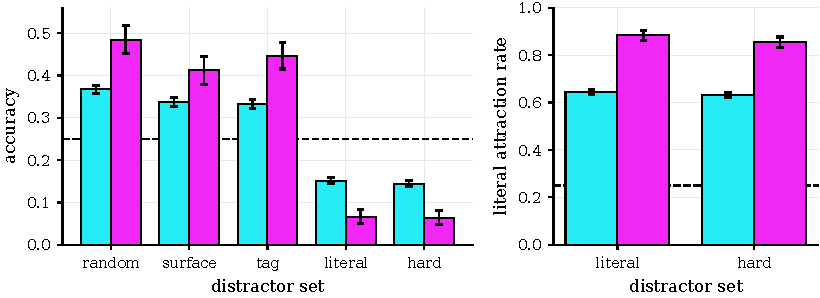
\includegraphics[width=0.90\linewidth]{figures/fig1_literal_capture.pdf}
\caption{The distractor ladder (left) and literal attraction rate (right) for
the two open arms. \swL Laya-ml ($n=8{,}876$), \swD Lod-lille ($n=888$);
the black dashed horizontal line marks the four-option chance level
($0.250$) in both panels; error bars are 95\% bootstrap CIs. Surface- and
tag-matched distractors cost a few points. Inserting the idiom's own literal
gloss (\Dlit) collapses both models far below chance, and collapses the
\emph{stronger} model harder: Lod-lille leads Laya-ml by $+0.133$ on random
distractors and trails it by $-0.070$ once the literal gloss is present.
On the right, both models select the literal reading over the figurative one
on the majority of items.}
\label{fig:ladder}
\end{figure*}




\begin{table}[t]
\centering\small
\renewcommand{\arraystretch}{1.12}
\begin{tabularx}{\columnwidth}{@{}>{\raggedright\arraybackslash}X>{\centering\arraybackslash}p{1.05cm}>{\centering\arraybackslash}p{1.05cm}>{\centering\arraybackslash}p{1.25cm}@{}}
\toprule
\textbf{Distractors} & \textbf{Laya} & \textbf{Lod} & $\boldsymbol{\Delta}$ \\
\midrule
random & 0.367 & \lodh{0.484} & \neu{$+0.133^{***}$} \\
surface & 0.338 & \lodh{0.412} & \neu{$+0.073^{***}$} \\
tag & 0.333 & \lodh{0.446} & \neu{$+0.120^{***}$} \\
\midrule
$+$ literal & \layah{0.151} & \lodh{0.066} & $-0.070^{***}$ \\
hard & \layah{0.144} & \lodh{0.063} & $-0.086^{***}$ \\
\midrule
\LAR{} (lit.) & 0.644 & \lodh{0.885} & \\
\LAR{} (hard) & 0.631 & \lodh{0.855} & \\
mean $p$(lit.) & 0.464 & \lodh{0.726} & \\
mean $p$(gold) & \layah{0.195} & 0.128 & \\
\bottomrule
\end{tabularx}
\caption{\textbf{The distractor ladder and literal attraction.}
McNemar tests use the 888 shared items ($^{***}$ $p<0.001$).
\textcolor{cLaya}{\rule[-0.05em]{0.7em}{0.7em}}\,Cyan marks
Laya-ml, while
\textcolor{cLod}{\rule[-0.05em]{0.7em}{0.7em}}\,magenta marks
Lod-lille; darker
\cellcolor{cLaya!55}\textbf{cyan} and
\cellcolor{cLod!42}\textbf{magenta}
fills highlight the higher value within a row.
The highlighted literal-bearing conditions and capture measures
expose the central pattern: adding the idiom's own literal gloss
causes a sharp accuracy drop and strong literal attraction.
The sign of $\Delta$ reverses at the literal boundary.}
\label{tab:ladder}
\end{table}

Within this pair, then, \LAR{} measures something accuracy does not: a model
can be selected as ``better'' on a conventional benchmark while being worse at
what that benchmark proxies for. Laya-ml and Lod-lille answer byte-identical questions in the same language, so
the crossover between them is a paired result. The error is not diffuse:
the decomposition under \Dlit{} is gold / literal / other $= 0.151$ / $0.644$ /
$0.207$ for Laya-ml and $0.066$ / $0.885$ / $0.048$ for Lod-lille, and on the
clearest items Laya-ml places $p = 1.000$ on the literal gloss.

\paragraph{Capture tracks the language, not capability.} The arms above ran
the literal condition in Bangla; the commercial arm's headline $\LAR = 0.047$
is \emph{English}, so the two are not comparable as they stand. We therefore
ran the full model $\times$ language matrix on the 3{,}265-item shared pool,
every cell built by one function from one seed
(Table~\ref{tab:matrix}, Figure~\ref{fig:matrix}). The English cell for
Jev-1.13 reproduces its published value at $0.0472$ $[0.0401, 0.0545]$, which
is the check that the two constructions measure the same thing.

Two things follow. First, \textbf{every arm is far more captured in Bangla than
in English on identical items}: $0.731 \rightarrow 0.379$, $0.918 \rightarrow
0.241$ and $0.304 \rightarrow 0.047$, all paired McNemar $p < 10^{-100}$. The
commercial model's apparent resistance to capture was a property of the language
it was tested in. Second, \textbf{capture is not monotone in capability}:
Lod-lille is more accurate than Laya-ml and more captured, while Jev-1.13 is more
accurate than both and less captured, so capability neither predicts capture nor
protects against it. The two open arms fall below chance here; Jev-1.13 does not,
but loses $0.390$ of accuracy against its own English run on the same items.
Appendix~\ref{app:matrix} gives the cells with intervals, and the caveat that the
pool is not a neutral sample.



\begin{figure}[t]
\centering
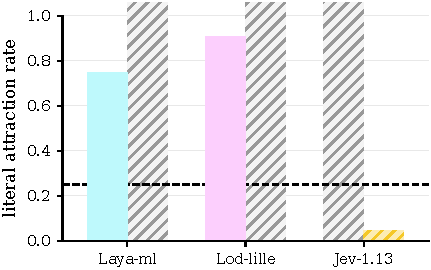
\includegraphics[width=\columnwidth]{figures/fig2_capture_matrix.pdf}
\caption{Literal attraction by model and task language, all six cells measured
on the same 3{,}265 items ($n=3{,}265$ each; error bars are 95\% bootstrap
CIs). The black dashed horizontal line marks the four-option chance level
($0.250$). \swL Laya-ml, \swD Lod-lille, and \swJ Jev-1.13; solid bars are
the Bangla condition, while hatched bars are the English condition. Every arm
is far more captured in Bangla than in English on identical items, and the
Bangla ordering does not follow capability: Jev-1.13 is the most accurate of
the three and the least captured, while Lod-lille is more accurate than
Laya-ml and the most captured. Jev-1.13's English value reproduces the figure
reported from its original run, $0.047$. Full numbers are given in
Table~\ref{tab:matrix}.}
\label{fig:matrix}
\end{figure}


\paragraph{The capability ordering.} One condition is identical across all three
arms, Bangla idiom with random distractors, and on it the commercial model is far
ahead, $0.736$ against $0.367$ and $0.484$ (Table~\ref{tab:threeway}). That is
the ordering against which the calibration results below should be read, and it
is the one capture does not follow.

\begin{table}[t]
\centering\small
\setlength{\tabcolsep}{4pt}
\begin{tabular}{lccc}
\toprule
\textbf{Model} & $n$ & \textbf{Accuracy} & \textbf{95\% CI} \\
\midrule
Laya-ml   & 8{,}876  & 0.367 & [0.357, 0.377] \\
Lod-lille & 888      & 0.484 & [0.453, 0.518] \\
Jev-1.13  & 8{,}761  & 0.736 & [0.727, 0.745] \\
\bottomrule
\end{tabular}
\caption{The only condition identical across all three arms: Bangla idiom
$\rightarrow$ Bangla gloss, random distractors. All pairwise McNemar tests on the
overlapping items are significant: Jev$-$Laya $+0.369$, Jev$-$Lod $+0.259$,
Lod$-$Laya $+0.133$ (all $p < 10^{-9}$).}
\label{tab:threeway}
\end{table}


\subsection{Confidence is anti-diagnostic}
\label{sec:confidence}

Table~\ref{tab:conf} gives the mean probability assigned to the chosen option,
split by outcome, on the literal-bearing families. Both open models are
\emph{more confident when captured than when correct}, Lod-lille extremely so
($0.787$ against $0.453$). The reliability curves in
Figure~\ref{fig:reliability} slope \emph{downward} under \Dlit{} in both.

\begin{table}[t]
\centering\small
\setlength{\tabcolsep}{4pt}
\begin{tabular}{lccc}
\toprule
\textbf{Outcome} & \textbf{Laya} & \textbf{Lod} & \textbf{Jev} \\
\midrule
correct          & 0.432 & 0.453 & \textbf{0.935} \\
captured         & \textbf{0.596} & \textbf{0.787} & 0.737 \\
other error      & 0.421 & 0.399 & 0.746 \\
\midrule
ECE (\Drand)     & 0.071 & 0.073 & 0.005 \\
ECE (\Dlit)      & 0.385 & 0.679 & 0.014 \\
AURC (conf.)     & 0.924 & 0.989 & 0.013 \\
AURC (random)    & 0.849 & 0.933 & 0.069 \\
\bottomrule
\end{tabular}
\caption{Confidence by outcome on the literal-bearing families, and calibration.
Bold marks, per model, whether the model is more confident when correct or when
captured. Both open arms are more confident when captured; their
confidence-gated AURC is \emph{worse} than the random-gate baseline in the grey
row, which inverts selective prediction. Jev-1.13's English condition does not
show the inversion.}
\label{tab:conf}
\end{table}

\begin{figure*}[t]
\centering
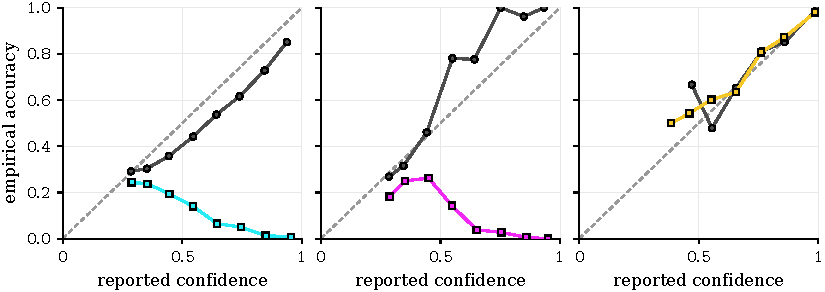
\includegraphics[width=0.90\linewidth]{figures/fig4_confidence_reliability.pdf}
\caption{Reliability, 15 equal-width bins. Panels left to right: \sw{cLaya}Laya-ml,
\sw{cLod}Lod-lille, \sw{cJev}Jev-1.13. \swK circles are the random-distractor
condition; squares in each panel's own colour are the $+$literal condition. The grey dashed
diagonal is perfect calibration. Under \Dlit{} the two open models' curves bend
\emph{downward}, higher stated confidence buying lower accuracy, while
Jev-1.13, running in English, stays on the diagonal. Reading the left two panels:
the model is most wrong exactly where it reports being most sure.}
\label{fig:reliability}
\end{figure*}

Selective prediction therefore inverts: restricting Laya-ml's \Dlit{} to its
most confident 5\% gives $0.007$ accuracy against $0.151$ at full coverage, and
Lod-lille answers every item in its most confident 35\% incorrectly
(Appendix~\ref{app:selective}). This is not an artifact of one calibration
philosophy. Laya-ml ships fitted per-bucket temperatures, Lod-lille ships none
by design, and Lod-lille's \emph{separate confidence head}, meant to estimate
whether the answer is in the option list at all, shows the same inversion
($0.631$ on captured items against $0.295$ on correct ones).

Jev-1.13 is the interesting exception, and it is only an exception in one
direction. Its reliability in English is close to ideal on the two families
in Table~\ref{tab:conf} (ECE $0.005$ and $0.014$, rising to $0.047$ on
\Dhard), and its confidence-gated AURC beats random by an order of
magnitude. That makes
\S\ref{sec:nosignal} harder to dismiss, not easier.

This does not contradict \citet{ibrahim2026evaluating}, who find
decision-model calibration better than most LLM baselines; we reproduce that for
the commercial arm on its own language. The narrower claim is that
in-distribution calibration need not survive a targeted distractor shift, and
that it fails in the costly direction: a confidence-gated cascade
\citep{li2026jevjudge} accepts the high-confidence tail without review, and on
the literal-bearing families that tail is where the open arms are \emph{least}
accurate.

\subsection{A semantics-free control, on all three arms}
\label{sec:nosignal}

The \textsc{o4} ablation replaces every option's text with a bare label. No
semantic signal remains, so with the gold position randomised the expected
accuracy is $0.25$ absent any signal, and whatever confidence survives is
overconfidence with no modelling assumption needed to read it. This is the only condition in the paper that runs
identically on all three arms: it requires no gloss, no literal annotation and
no shared language, so the language confound that scopes
\S\ref{sec:capture}--\S\ref{sec:confidence} to the two open arms does not
arise here. Figure~\ref{fig:nosignal} reports it.


\begin{figure}[t]
\centering
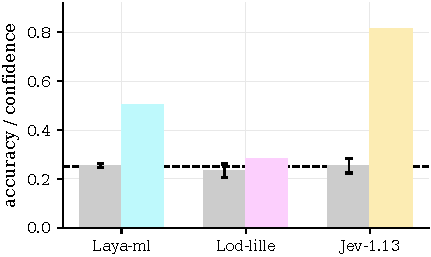
\includegraphics[width=\columnwidth]{figures/fig5_no_signal_control.pdf}
\caption{The semantics-free control. Per model, the \swG bar is accuracy
(with 95\% bootstrap CI) and the coloured bar is mean reported confidence
(\swL Laya-ml, \swD Lod-lille, \swJ Jev-1.13). The black dashed horizontal
line marks the four-option chance level ($0.250$). Because the options carry
no information, accuracy is at chance by construction and the gap between
confidence and accuracy is pure overconfidence: $0.250$ for Laya-ml,
$0.049$ for Lod-lille, and $0.561$ for Jev-1.13, which reports $0.815$
confidence while answering at $0.254$. Jev-1.13's condition is English.}
\label{fig:nosignal}
\end{figure}

The ordering reverses against Table~\ref{tab:conf}. The best-calibrated model
under real options is the worst when the options carry nothing: Jev-1.13 reports
$0.815$ mean confidence at $0.254$ accuracy, an ECE of $0.561$. Lod-lille, the
weakest of the three on accuracy, is the only one whose reported confidence
collapses appropriately ($0.282$). We read this as the most portable finding in the
paper, because it is the one that needs no annotation and no matched language to
reproduce: a calibration number measured on in-distribution options says little
about what a model will report when the option list is degenerate, and a caller
thresholding on a returned probability is exposed to that case. Confidence-based acceptance is the mechanism of the cascade
designs proposed for this class \citep{li2026jevjudge,ibrahim2026evaluating},
and a degenerate option list is an ordinary consequence of an upstream bug or an
empty retrieval rather than an adversarial construction.

A side-check comes with it: McNemar between the two open arms under \textsc{o4}
is not significant ($p = 0.76$), so the instrument's null behaves identically in
both.

\subsection{Option order is architecture-specific}
\label{sec:order}

We run every item under all $4! = 24$ orderings of a fixed option set and record
the identity of the chosen gloss, recovered as $\mathrm{perm}[\mathrm{slot}(\hat{y})]$.\footnote{%
An earlier version of this analysis counted distinct option \emph{keys} (slot
letters) and reported near-total instability for Laya-ml. That metric is an
artifact: a key necessarily changes when the same gloss moves slots. All numbers
here use the corrected gloss-identity metric; Laya-ml's figure drops from $1.000$
to $0.837$ and the finding stands.}

\begin{table}[t]
\centering\small
\renewcommand{\arraystretch}{1.12}
\begin{tabularx}{\columnwidth}{@{}>{\raggedright\arraybackslash}X>{\centering\arraybackslash}p{1.05cm}>{\centering\arraybackslash}p{1.05cm}>{\centering\arraybackslash}p{1.05cm}@{}}
\toprule
& \textbf{Laya} & \textbf{Lod} & \textbf{Jev} \\
\midrule
answer changes      & \textbf{0.837} & 0.107 & 0.133 \\
correctness varies  & \textbf{0.686} & 0.070 & 0.120 \\
distinct glosses    & \textbf{2.83}  & 1.14  & 1.15  \\
perfectly stable    & 0.163 & \textbf{0.893} & 0.867 \\
$p$(gold) range     & \textbf{0.346} & 0.029 & 0.128 \\
selection spread    & \textbf{0.226} & 0.052 & 0.072 \\
\bottomrule
\end{tabularx}
\caption{\textbf{Option-order sensitivity.}
Each item is evaluated under all 24 orderings of the same four options
($n=992/299/300$ items for Laya, Lod, and Jev, respectively).
\textcolor{cLaya}{\rule[-0.05em]{0.7em}{0.7em}}\,Laya,
\textcolor{cLod}{\rule[-0.05em]{0.7em}{0.7em}}\,Lod, and
\textcolor{cJev}{\rule[-0.05em]{0.7em}{0.7em}}\,Jev identify the three
model arms. Bold marks the largest value in each row. The marker-based
scorer changes its chosen gloss on 83.7\% of items, while the
independent-option scorer changes it on 10.7\%. Lod is documented as
order-independent by construction; the audit in
Appendix~\ref{app:position} shows that it is not, which is why its
entries here are small rather than zero.}
\label{tab:order}
\end{table}

Table~\ref{tab:order} gives a large dissociation: a $7.8\times$ difference in
answer stability and a $12\times$ difference in probability stability. Each
scoring design is represented by exactly one model here, so the design cannot be
separated from the backbone or the capability of the model carrying it; we read
the pattern as consistent with the scoring architecture rather than as
demonstrated to follow from it.

\paragraph{The invariance claim does not hold.} Lod-lille's design is documented
as order-independent by construction: each option is scored in its own forward
pass, so permuting the list should return identical probabilities. Mapping every
slot's returned probability back to the option that slot displayed, we can ask
how far a \emph{single} option's own score travels across the 24 orderings of its
list. At the median item it travels $4.0 \times 10^{-2}$, and on none of the 299
items does it stay below $10^{-4}$ (Appendix~\ref{app:position}). That is orders
of magnitude above \texttt{fp32} accumulation noise, so the residual instability
in Table~\ref{tab:order} is not a tie-breaking or slot-indexing artifact of our
harness; the scores themselves move. The reading we take is the narrow one: the
independent-option design attenuates order dependence substantially, by roughly
an order of magnitude against the marker-based scorer, but it does not remove it,
and an evaluation resting on the documented guarantee would be resting on
something we could not reproduce.



Positional bias follows. With the gold placed uniformly, Laya-ml takes slot B
37.2\% of the time against 14.6\% for slot A, a $2.6\times$ accuracy swing from
position alone (Appendix~\ref{app:position}).

\paragraph{Methodological consequence.} Any evaluation of this class that fixes
option order is partly measuring position. All results here randomise order per
item, seeded by item id, and are averages over position rather than measurements
at one of them; on the evidence here we would treat randomising order as a
default for this class rather than as a robustness check.

\subsection{Options are read as a bag of words}
\label{sec:bagofwords}

The \textsc{o}-series ablates the option text while holding the idiom fixed
(Figure~\ref{fig:options}; Table~\ref{tab:bnmanip} shows the forms applied to
real Bangla). Truncating each option to six words and \emph{scrambling the words
inside it} cost almost nothing: Laya-ml retains $0.967$ and $0.925$ of its
signal, Lod-lille $0.909$ and $0.948$, Jev-1.13 is flat to within noise. What
all three do on the option side is, behaviourally, close to order-free lexical
matching; we observe the invariance and do not claim to have identified the
mechanism producing it. The
drop to the grey semantics-free bar is the only large one, which certifies the
instrument: the task measures option semantics, as a bag.

This converges with \citet{sun2026typesafe}, who permute which option name is
bound to which definition and find the decision follows the name: within an
option, these models read lexical identity rather than composed meaning.


\subsection{Neither open model treats the idiom as a unit}
\label{sec:unit}

E3 perturbs the idiom while holding the option list fixed
(Figure~\ref{fig:unit}). This is the experiment that stands in for token
attribution: rather than asking what each word contributes, which presumes a
decomposition the expression may not support, we ask whether the model behaves as
though it stores the expression as a unit. A model that did would lose the
figurative reading when the unit is broken.

Neither does. Word-shuffling leaves Laya-ml's accuracy statistically unchanged
($0.158 \rightarrow 0.168$) and reversal helps slightly ($0.180$); Lod-lille
moves within noise. Agreement with the intact answer under shuffling is $0.742$
and $0.917$, so Lod-lille is more \emph{stable} but no more
\emph{compositional}. Table~\ref{tab:bnmanip} shows the perturbed strings.

The one manipulation that clearly helps both is embedding the idiom in its gold
carrier sentence, $+0.080$ and $+0.117$: context, not the idiom string, carries
the usable signal. The pattern is consistent with these models matching
whatever lexical material is available rather than retrieving a stored figurative
entry, though E3 can rule out unit storage without establishing what replaces it.
That cuts both ways, since \citet{xu2026jevout} flip 61.4\% of initially correct
decisions with short, fluent additions chosen to redirect the decision, and
nothing in the interface distinguishes a helpful addition from a harmful one.


\subsection{The failure localises to Bangla, in every arm}
\label{sec:crosslingual}

Holding the model fixed and swapping the task language
(Figure~\ref{fig:crosslingual}) moves every arm by a large margin: Laya-ml
$+0.246$, Lod-lille $+0.380$, Jev-1.13 $+0.233$ (all McNemar $p < 0.001$). As in
the matrix, the English condition presents the annotator's nearest English idiom
rather than a translation, so this is a comparison between paired entries;
Appendix~\ref{app:construction} sets out what that does and does not license.
Lod-lille reaches $0.864$ in English against $0.484$ in Bangla, so the figurative
concepts appear to be largely available to it, and the Bangla route is where the
loss occurs. Its documentation states that training evaluation was English-only,
which is consistent with what we see from outside the model.

Laya-ml's control arm supports this reading: its English-only checkpoint run on
Bengali script sits at $0.283$, barely above chance, which reproduces a
documented failure mode and makes it unlikely that the Bangla result is an
artifact of the scorer rather than of the language.

The two language cells are paired entries rather than identical items, and
their literal glosses are built from one annotated field by different routes;
Appendix~\ref{app:construction} documents the asymmetries and shows the capture
gap survives on the subset where the largest of them cannot operate.

Jev-1.13 complicates the reading and then confirms it. A model with no
multilingual claim outscores both that have one on the Bangla task, so the gap is
reachable rather than intrinsic to the script; yet its own literal attraction
rises from $0.047$ to $0.304$ when the same items are asked in Bangla. Being
better at a language is not the same as being robust in it, and the penalty
reaches every arm we tested.


\section{Discussion}

The matrix in \S\ref{sec:capture} is the result we would defend hardest,
because it separates two explanations that are easy to conflate. Read only in
English, the commercial arm looks immune to literal capture; read in Bangla on
the same items it is captured at six times the rate. What a decision model does
with a non-compositional expression is therefore not a fixed property of the
model, and a benchmark run in one language will not tell you how it behaves in
another. Capability does not order the failure either: the strongest arm is the
least captured, the middle arm the most.

The other results sit at different scopes and are worth keeping apart. The
semantics-free control runs identically on all three arms and needs no
annotation or shared language, so it is the one we would most expect to
transfer. The confidence inversion is a paired result on the two open arms.
Option-order dependence tracks the scoring architecture rather than the model,
and is the one place our audit confirms a design claim rather than denting
one.

For practitioners we would draw three cautions rather than
recommendations: a returned probability is worth little without a measurement of
what the model returns on a degenerate option list; a benchmark score is not by
itself evidence against literal capture, since on our two open arms the two move
in opposite directions; and an evaluation that fixes option order is partly
reporting position.

This is a boundary condition rather than a rebuttal: the cost and latency
advantages are established \citep{tang2026audit,rao2026rubric}, and what we add
is that the property the cascade designs depend on degrades first and silently.
The typed interface guarantees a well-formed answer and nothing about whether it
was arrived at for a reason, so each of these failures is invisible to a caller
who only checks that the output validates.

\section{Conclusion}

We audited three decision models on Bangla idioms using only interventions on
the option set, a method that needs no annotation and stays available when a
model emits no text and its weights are closed. Replacing one distractor with an
idiom's own expert literal gloss captures all three, and running the full model
$\times$ language matrix on a shared 3{,}265-item pool shows what the failure
tracks: literal attraction falls from $0.731$, $0.918$ and $0.304$ in Bangla to
$0.379$, $0.241$ and $0.047$ in English, so the commercial arm's apparent
resistance belongs to the language it was tested in rather than to the model.
Capability does not order the failure, since the strongest arm is the least
captured and the middle arm the most. Confidence inverts under the same shift,
and with the options stripped of semantics, where accuracy is pinned at chance,
the arms still report between $0.28$ and $0.82$ confidence. Option-order
sensitivity separates the two scoring architectures rather than the three
models. The instrument costs no annotation and, for the commercial arm, about
eleven cents to run; we release it so the same audit can be pointed at other
models and other languages.

\section*{Limitations}

All three models are evaluated zero-shot, and this is the limitation we would
weigh most heavily after the one below. Decision models are trained on a
particular set of decision tasks, and the open arms' own documentation reports
that base checkpoints are weak on tasks outside that set. Some part of what we
measure may therefore be out-of-distribution task transfer rather than literal
capture specifically. The \textsc{o4} control bounds this from one side, since
it shows the instrument's null behaving identically in both open arms, and the
\Drand{} to \Dlit{} contrast is within-model and within-item, which removes any
fixed task-transfer offset. Neither argument rules the confound out. A single
lightly fine-tuned arm would settle it, and we have not run one.

Laya-ml's run had its per-bucket temperatures unset, so its ECE figures are raw.
Lod-lille ships no temperature by design, so both open arms are effectively
untempered and comparable on that axis; Jev-1.13's internal calibration is
unknown to us.

Lod-lille ran a fixed 10\% subset (888 items), so its intervals are roughly
$\pm 3$ points and its stratified cells are thin. Appendix~\ref{app:subset}
bounds the subset bias at $0.016$ and shows it changes no sign or ordering. E3
on the Lod-lille arm is 180 items and several of its perturbation contrasts are
not individually significant. E7 covers 992 / 299 / 300 items rather than the
full sets.

The matrix in \S\ref{sec:capture} runs on the 3{,}265 items that carry a
usable English literal gloss, which is not a neutral sample: for Laya-ml,
in-pool \LAR{} is higher than out-of-pool while \Drand{} accuracy is
unchanged, so the absolute rates there are higher than they would be corpus
wide. The language comparison is paired within item and within model, so that
selection affects the levels rather than the direction. The matrix also covers
the literal condition only; we did not run the other distractor families in both
languages. The confidence results in \S\ref{sec:confidence} remain two-arm,
since the commercial arm's reliability was measured on its English run.

The two language cells are also not symmetric in construction, and this is the
limitation we would flag hardest. They are paired entries rather than identical
items: the Bangla state is the idiom, while the English state is the annotator's
nearest English idiom rather than a translation of it. The two literal glosses are
drawn from one annotated field in different ways, and the resulting Bangla gloss
shares a content word with its own state on $56.2\%$ of pool items against
$25.1\%$ on the English side, which hands a lexical matcher a surface hook in
Bangla that it does not have in English. Appendix~\ref{app:construction} sets out
all four asymmetries we could find and tests this one directly: restricted to the
$1{,}429$ items where the Bangla literal gloss shares no content word with the
idiom, the capture gap is $+0.358$, $+0.610$ and $+0.310$ for the three arms,
against headline gaps of $+0.352$, $+0.677$ and $+0.256$. The hook therefore does
not account for the result, but we cannot rule out smaller construction effects of
the same kind, and a properly translation-paired corpus would settle what we can
only bound.

More broadly, this is one corpus, one language, two small open models and one
commercial endpoint. The semantics-free control is the only result here that we
would expect to transfer as stated; the rest should be read as findings about
these systems on this material, and as an instrument other people can point at
theirs.

Distractors are drawn from the same corpus, so difficulty is corpus-relative
rather than absolute. Jev-1.13 is a commercial endpoint and may change without
notice; our results are a snapshot, and we report the exact call count and cost
in Appendix~\ref{app:repro} so the snapshot is at least auditable.


\section*{Ethics Statement}

The corpus is a published, expert-annotated resource of idioms \citep{sakhawat-etal-2026-words}; it contains no
personal data and no content about identifiable individuals. Our interventions
rewrite option lists and perturb idiom strings, and produce no new annotation and
no generated text.

The work audits two openly released models and one commercial API. We report
failure modes in all three, including the vendor's. We have taken care to
separate what is measured from what is inferred. An earlier version of this
work reported the commercial arm's low literal attraction without running it in
Bangla; completing the matrix showed that result was a property of the test
language, and \S\ref{sec:capture} now reports the corrected picture rather
than the flattering one. \S\ref{sec:capture} also states the pool selection
effect against our own cleanest number. Commercial endpoints are
mutable; readers should treat the Jev-1.13 results as dated rather than as a
standing property of the product.

Bangla is under-served relative to its speaker population, and we think an audit
that locates a failure in the language rather than in the task is the more useful
kind to publish. The instrument, the per-item outputs and the analysis code are released; Appendix~\ref{app:repro} is the run record they correspond to.

\bibliography{references,custom}

\appendix

\section{The typed question}
\label{app:payload}

Every call in this paper sends one typed \texttt{choice} question and receives
one probability vector. Nothing else is exchanged: there is no prompt template,
no system message, no sampling parameter and no generated text. This is the
whole interface, which is why the option set is the only intervention surface
available.

\paragraph{Request.} For the commercial arm the body posted to
\texttt{/api/alpha/decisions} is

\begin{quote}\footnotesize\ttfamily
\{"model": "typesafe/jev-1.13",\\
\ "state": \textit{<idiom, or carrier sentence>},\\
\ "questions": \{"q": \{\\
\ \ \ "type": "choice",\\
\ \ \ "instructions": \textit{<one sentence, Table~\ref{tab:instr}>},\\
\ \ \ "criteria": \{"A": \textit{<gloss>}, "B": \textit{<gloss>},\\
\ \ \ \ \ \ \ \ \ \ \ \ \ \ \ "C": \textit{<gloss>}, "D": \textit{<gloss>}\}\}\}\}
\end{quote}

The two open arms are called locally with the same four fields: the idiom as
state, the instruction string, and the four option texts keyed \texttt{A}--%
\texttt{D}. The option order is shuffled per item by a generator seeded with the
item id and the experiment seed, so the same item receives the same permutation
in every arm and every family.

\paragraph{Response.}

\begin{quote}\footnotesize\ttfamily
\{"type": "choice", "choice": "B", "confidence": 0.75,\\
\ "probabilities": \{"A": 0.00, "B": 0.84,\\
\ \ \ \ \ \ \ \ \ \ \ \ \ \ \ \ \ \ \ "C": 0.16, "D": 0.00\}\}
\end{quote}

We assert on every call that the returned keys are a subset of
\texttt{\{A,B,C,D\}} and that the probabilities sum to $1$ within $10^{-2}$; no
call in any run violated either.

\paragraph{Two confidence signals, and which one we use.} Note that
\texttt{confidence} is not the maximum probability: in the example above it is
$0.75$ while $\max_o p(o) = 0.84$. It is a separate head whose documented job is
to estimate whether the correct answer is present in the option list at all.
Lod-lille ships the same arrangement. We log it as \texttt{conf\_head} and
report it where it matters (\S\ref{sec:confidence}), but every cross-model
number in this paper uses the maximum probability, because it is the only
confidence signal all three arms define identically. Where the two disagree the
head is not the more diagnostic of the pair: on Lod-lille's captured items mean
head confidence is $0.631$ against $0.295$ on correct ones, the same inversion
the top probability shows.

\paragraph{Answer types we did not use.} The interface also accepts
\texttt{score} (a bounded numeric judgement) and \texttt{boolean} questions. We
use \texttt{choice} exclusively and deliberately. A \texttt{score} question
would ask the model to rate a gloss in isolation, which destroys the property
the instrument depends on: that the gold and the literal reading compete inside
a single forward pass, exactly as the psycholinguistic account describes
\citep{cacciari1988comprehension,titone1999compositional}. A \texttt{boolean}
question would do the same and additionally reintroduce a yes/no label whose
name carries meaning of its own, which is the failure
\citet{sun2026typesafe} document. Keeping every experiment in one answer type
also means the five distractor families differ in nothing but their option text.

\begin{table}[t]
\centering\small
\renewcommand{\arraystretch}{1.12}
\begin{tabularx}{\columnwidth}{@{}>{\raggedright\arraybackslash}p{1.35cm}>{\raggedright\arraybackslash}X@{}}
\toprule
\textbf{Arm} & \textbf{Instruction string} \\
\midrule
Laya-ml &
Bangla, see note \\
Lod-lille &
Bangla, identical to above \\
Jev-1.13 &
``What is the actual figurative meaning of this idiom?'' \\
\bottomrule
\end{tabularx}
\caption{The instruction is one sentence and is byte-identical across families,
experiments and the two Bangla arms. The Bangla string is the direct equivalent
of the English one.}
\label{tab:instr}
\end{table}

\section{Positioning against concurrent work}
\label{app:positioning}

The decision-model literature is a few weeks old at the time of writing, and
several papers describe failures adjacent to ours. This appendix states what
each one establishes, what it does not, and why our design is complementary
rather than duplicative.

\paragraph{Mechanism versus behaviour.} \citet{oh2026tug} apply causal tracing
to autoregressive transformers and recover two pathways carrying an idiom's
figurative and literal readings at once: early layers and specific attention
heads promote the figurative interpretation while a direct route keeps the
literal one available, and disambiguating context is integrated from the first
layer onward. That is mechanistic evidence that the competition our \Dlit{}
condition exploits is real inside a model, and it is what makes our outcome
measure interpretable rather than arbitrary: when a decision model places its
mass on the literal gloss, there is a documented sense in which both readings
were present and one won.

The two designs answer different questions, and the difference is the reason
both are needed. Causal tracing requires weight access, token-level activations
and a generative forward pass to intervene on. None of the three systems we
audit offers the first, two of them emit no token stream to trace, and one is a
commercial endpoint behind an HTTP interface. Their method cannot be pointed at
the systems that are currently being deployed as routers and guardrails; ours
can, at the cost of saying nothing about where inside the model the competition
is resolved. They establish \emph{how} the literal route survives; we measure
\emph{how often} it takes over, in which language, and with what confidence
attached.

\paragraph{Option names and option definitions.} \citet{sun2026typesafe} hold a
typed model's option definitions fixed and permute which name is bound to which,
and find decision-flip rates up to 70.4 points higher for semantically loaded
labels than for neutral ones: the model follows the name rather than the
definition it was given. They note that type-safety conceals this, because every
output remains structurally valid.

Our \textsc{o}-series (\S\ref{sec:bagofwords}) manipulates the complementary
half. We hold the option names fixed at \texttt{A}--\texttt{D} and destroy the
internal structure of the text bound to them, by truncation and by shuffling
words within each option, and find accuracy almost unchanged. Read together, the
two results bracket the same conclusion from either side: within an option,
these models are sensitive to lexical identity and insensitive to composed
meaning. Neither result alone would establish that, because theirs is consistent
with a model that reads definitions carefully but weights names more heavily,
and ours is consistent with a model that reads definitions as unordered bags.

\paragraph{Context that flips decisions.} \citet{xu2026jevout} append short,
fluent, task-preserving context and redirect 61.4\% of initially correct
decisions, with targeted flip rates of 64.9--73.2\% across systems. Our E3
carrier-sentence condition (\S\ref{sec:unit}) is the benign case of the same
mechanism: embedding an idiom in its gold example sentence \emph{raises}
accuracy by $0.080$ and $0.117$ on the two open arms. The two findings are the
same sensitivity with opposite signs, and the uncomfortable implication is that
a caller cannot tell them apart from the interface. A model whose answer
improves when helpful context is appended is, necessarily, a model whose answer
moves when context is appended at all.

\paragraph{Calibration and cascades.} \citet{ibrahim2026evaluating} evaluate
decision models against 19 language models on 18 computational social science
tasks, and report a median deficit of 11.6 F1 at 44 times lower cost, with
confidence calibration \emph{exceeding} most baselines; they recommend
decision models as a cheap first stage that routes uncertain items onward.
\citet{li2026jevjudge} build that system, accepting high-confidence verdicts and
escalating the rest, and exceed a frontier model's accuracy at 41\% of its cost.

We reproduce the favourable calibration for the commercial arm on its own
language (\S\ref{sec:confidence}), so this is not a contradiction. The boundary
we add has two parts. First, in-distribution calibration does not survive a
targeted distractor shift, and it fails in the direction that costs a cascade
most: on the literal-bearing families the high-confidence tail is where the open
arms are \emph{least} accurate, so a confidence gate forwards exactly the items
that should have been escalated. Second, and independent of any distribution
assumption, the semantics-free control (\S\ref{sec:nosignal}) shows what each
arm reports when the option list provably carries no information. A gate
calibrated on real options has no defence against that case, and a degenerate
option list is an ordinary consequence of an upstream bug or an empty retrieval.

\paragraph{What none of this settles.} All of the above, ours included, is
zero-shot evaluation of base checkpoints. \citet{tang2026audit} review 28 papers
published within nine days of the first widely used release and conclude that
the typed readout has shown no independent accuracy advantage, with the
demonstrated gains in latency, cost and cascade placement. Whether any of these
failure modes survives task-specific fine-tuning is, as far as we can determine,
unmeasured by anyone so far.


% \begin{figure*}[t]
% \centering
% 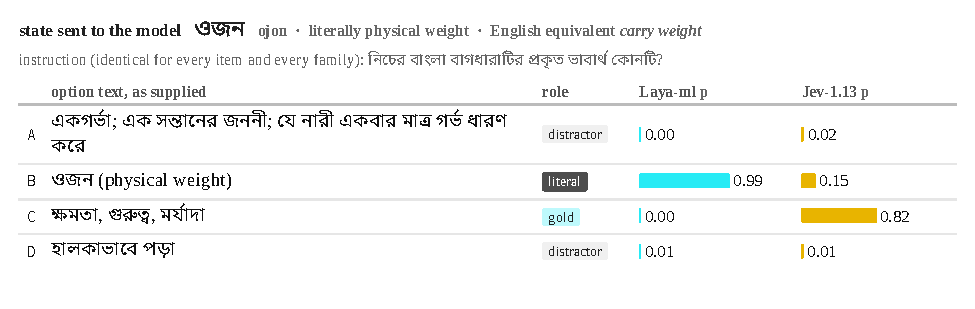
\includegraphics[width=\linewidth]{figures/fig_bn_item.pdf}
% \caption{One item exactly as the two models received it, in the original
% Bengali script. The state is the idiom \emph{ojon}; the four option texts are
% the real ones, reconstructed with the builder and seed the run used and checked
% against the recorded gold and literal keys. The probabilities are the returned
% values. Laya-ml places $0.99$ on the \textbf{literal} option, which names the
% weight of an object, and $0.00$ on the gold figurative gloss; Jev-1.13 places
% $0.82$ on the gold. This figure was rendered outside \LaTeX{} because pdf\LaTeX{}
% cannot shape Bengali; it is vector, with embedded font subsets and selectable
% text.}
% \label{fig:bnitem}
% \end{figure*}


\begin{table*}[t]
\centering
\small

\begin{tabularx}{\textwidth}{
    @{}
    c
    >{\raggedright\arraybackslash}X
    >{\centering\arraybackslash}p{1.45cm}
    >{\centering\arraybackslash}p{1.55cm}
    >{\centering\arraybackslash}p{1.55cm}
    @{}
}
\toprule

&
\textbf{option text, as supplied}
&
\textbf{role}
&
\textbf{Laya-ml $p$}
&
\textbf{Jev-1.13 $p$}
\\
\midrule

A &
\bangla{একগর্ভা; এক সন্তানের জননী; যে নারী একবার মাত্র গর্ভ ধারণ করে} &
\textit{distractor} &
0.00 &
0.02
\\[3pt]

B &
\bangla{ওজন} (\emph{physical weight}) &
\textbf{literal} &
\pL{0.99} &
\pJ{0.15}
\\[3pt]

C &
\bangla{ক্ষমতা, গুরুত্ব, মর্যাদা} &
\textbf{gold} &
0.00 &
\pJ{0.82}
\\[3pt]

D &
\bangla{হালকাভাবে পড়া} &
\textit{distractor} &
0.01 &
0.01
\\

\bottomrule
\end{tabularx}

\caption{\textbf{One item exactly as received by the models.}
The state is the Bangla idiom \bangla{ওজন} (\emph{ojon}), literally
``physical weight,'' with the English equivalent \emph{carry weight}.
The instruction is identical across items and distractor families.
The four option texts are the actual strings reconstructed with the
builder and seed used for the run and checked against the recorded gold
and literal keys. The probabilities are the returned values. Laya-ml
places $0.99$ on the literal option, which denotes the physical weight
of an object, and $0.00$ on the gold figurative gloss; Jev-1.13 places
$0.82$ on the gold option.}
\label{tab:bnitem}

\end{table*}




\section{What each experiment changes}
\label{app:experiments}

Table~\ref{tab:expgrid} states, for each experiment, the one thing that varies
and the things held fixed. Reading down the ``varies'' column follows the
argument: each row isolates one candidate explanation for the failure measured
in E1.

\begin{table}[h]
\centering\small
\setlength{\tabcolsep}{3pt}
\begin{tabular}{llll}
\toprule
& \textbf{Varies} & \textbf{Fixed} & \textbf{Seed} \\
\midrule
\neu{E1} & \neu{distractors} & \neu{idiom, instr., $k$} & \neu{1000} \\
E2 & idiom surface & meaning, options & 2000 \\
E3 & idiom form & options, instr. & 3000 \\
E4 & task language & item, family & 4000 \\
\neu{E5} & \neu{nothing (derived)} & \neu{n/a} & \neu{n/a} \\
E6 & option text & idiom, gold & 6000 \\
E7 & option order & option set & 7000 \\
\bottomrule
\end{tabular}
\caption{The seven interventions. E5 issues no calls of its own; it is computed
from the E1 outputs. Seeds are the Bangla arms'; the commercial arm uses a
disjoint set (Appendix~\ref{app:repro}) because its blocks were run in a
different order.}
\label{tab:expgrid}
\end{table}

\paragraph{E1, the ladder.} \Drand{} samples three other idioms' figurative
glosses uniformly. \Dsurf{} samples glosses sharing at least one surface token
with the gold. \Dsem{} samples glosses from idioms sharing at least one semantic
tag. \Dlit{} replaces one sampled distractor with the idiom's own expert literal
gloss. \Dhard{} applies all three pressures at once. Duplicates are removed and
the slate is topped up from the random pool if fewer than $k$ distinct options
survive.

\paragraph{E3, perturbing the unit.} E3 runs on the literal-bearing option set,
so its accuracies are comparable to \Dlit{} rather than to \Drand: on the same
1{,}778 items Laya-ml scores $0.176$ under \Dlit{} and $0.353$ under \Drand,
against $0.158$ for the intact idiom here. \textsc{v0} is the intact idiom.
\textsc{v1} shuffles its words, \textsc{v2} reverses them, \textsc{v3} deletes
one word at random, \textsc{v4} substitutes one word with a word sampled from
another idiom, and \textsc{v5} replaces the idiom with its gold carrier
sentence. The option list is held byte-identical across all six, so the only
difference reaching the model is the state string.

\paragraph{E6, ablating the options.} \textsc{o0} is the full gloss. \textsc{o1}
truncates every option to its first six words. \textsc{o2} shuffles the words
within each option. \textsc{o3} replaces each gloss with its counterpart in the
other language. \textsc{o4} replaces every option with a bare label carrying no
semantics, which pins accuracy at chance by construction and is the control of
\S\ref{sec:nosignal}.

\section{Why interventions on the option set}
\label{app:why}

This appendix explains the design choice the rest of the paper rests on, for
readers who want the reasoning rather than the result.

A decision model takes a question and a list of candidate options and returns a
probability over exactly those options. It is not autoregressive, it does not
sample, and it emits no text. Three of the usual explainability routes are
therefore closed. There is no rationale to inspect and no chain of thought whose
faithfulness could be measured \citep{jacovi2020faithfulness,turpin2023unfaithful}.
Weights are available for two of our arms but not for the commercial one, so no
method that requires opening every model, including probing and causal tracing,
can be applied uniformly across the three \citep{oh2026tug}. And input attribution, the usual
fallback \citep{ribeiro2016lime,lundberg2017shap}, is not only unreliable here
\citep{jain2019attention,adebayo2018sanity,hooker2019roar} but hard to interpret
for this material.

The last point needs stating carefully, because it is what motivates everything
else, and the standard shorthand for it is too strong. Idioms are not uniformly
non-compositional. \citet{nunberg1994idioms} argue the opposite of the slogan
usually attributed to them: idioms vary in how far their parts can be mapped onto
components of the figurative reading, and many are \emph{idiomatically
decomposable}, with \emph{spill the beans} distributing its meaning across
\emph{spill} and \emph{beans} in a way that \emph{kick the bucket} does not.
Psycholinguistic work finds decomposability measurable and consequential for
processing \citep{gibbs1989kick,titone1999compositional}.

What follows is weaker than ill-posedness but enough for our purposes. A Shapley
value over the tokens of an idiom is always computable, and for a
non-decomposable expression there is no reason to expect the resulting per-token
shares to correspond to anything linguistically real: the quantity is defined by
the attribution game rather than by a decomposition the expression actually
supports, and decomposability is a property of the individual idiom that we do not
have annotated. The numbers will still arrive, and they will still read as an
explanation. We therefore do not build on them, and intervene on the interface
instead, which requires no assumption about where an idiom's meaning sits.

What remains is the interface itself. The caller controls the question and the
option list and observes a probability vector. So we intervene there. The
corpus supplies, for every idiom, both a gold figurative gloss and an expert
literal gloss, which means a counterfactual distractor is already annotated and
we create no new labels: dropping the literal gloss into the option list turns a
benchmark item into a targeted probe of whether the expression was read as an
idiom or as its words. Holding the item, the instruction and $k$ fixed while
varying only the distractor family makes the comparison within-item and
within-model, so a difference between two families cannot be explained by item
difficulty, by the prompt, or by anything about the model that does not change
between the two calls.

The same logic produces the other six interventions. If the failure were about
the idiom's surface form rather than its meaning, E2 would show it. If the model
held the expression as a stored unit, breaking the unit in E3 would hurt. If the
problem were figurativeness rather than the language, E4 would not move. If the
model read options as sentences rather than as bags of words, E6 would collapse
under scrambling. If the scorer were order-independent as documented, E7 would
return the same gloss under all 24 permutations. Each experiment is an attempt
to explain the E1 result away, and the paper reports which attempts succeed.

\section{The full distractor ladder}
\label{app:ladder}

Table~\ref{tab:fullladder} gives every family for every arm. Two caveats on the
commercial column: its numbers are English, and its \Dsurf{} and \Dsem{} rows
run on the larger 8{,}761-item English pool rather than the 3{,}265-item
literal pool, because those families need no literal gloss.

\begin{table}[t]
\centering\small
\renewcommand{\arraystretch}{1.12}
\begin{tabularx}{\columnwidth}{@{}>{\raggedright\arraybackslash}X>{\centering\arraybackslash}p{1.35cm}>{\centering\arraybackslash}p{1.35cm}>{\centering\arraybackslash}p{1.35cm}@{}}
\toprule
\textbf{Family} & \textbf{Laya-ml} & \textbf{Lod-lille} & \textbf{Jev-1.13} \\
& bn & bn & en \\
\midrule
\Drand & 0.367 & 0.484 & 0.968 \\
\Dsurf & 0.338 & 0.412 & 0.915 \\
\Dsem  & 0.333 & 0.446 & 0.829 \\
\Dlit  & 0.151 & 0.066 & 0.931 \\
\Dhard & 0.144 & 0.063 & 0.854 \\
\midrule
\LAR{} \Dlit  & 0.644 & 0.885 & 0.047 \\
\LAR{} \Dhard & 0.630 & 0.855 & 0.043 \\
\bottomrule
\end{tabularx}
\caption{Accuracy by distractor family, and literal attraction on the two
families that contain a literal gloss. Chance is $0.250$. The commercial column
is English and is the reason \S\ref{sec:capture} runs the matrix: compare it
with the Bangla column of Table~\ref{tab:matrix}, where the same model is
captured at $0.304$.}
\label{tab:fullladder}
\end{table}

\section{Selective prediction in detail}
\label{app:selective}

Selective prediction asks what happens if the caller answers only the items the
model is most confident about. A useful confidence signal makes accuracy rise as
coverage falls. Table~\ref{tab:riskcov} reports accuracy at low coverage for the
two open arms, on the random-distractor condition and on the literal-bearing
one.

\begin{table}[t]
\centering\small
\renewcommand{\arraystretch}{1.12}
\begin{tabularx}{\columnwidth}{@{}>{\raggedright\arraybackslash}p{1.05cm}*{4}{>{\centering\arraybackslash}X}@{}}
\toprule
\textbf{Coverage} &
\laya{\textbf{\Drand}} &
\laya{\textbf{\Dlit}} &
\lod{\textbf{\Drand}} &
\lod{\textbf{\Dlit}} \\
\midrule
0.05 & \laya{0.669} & \laya{0.007} & \lod{0.977} & \lodh{0.000} \\
0.10 & \laya{0.597} & \laya{0.007} & \lod{0.989} & \lodh{0.000} \\
0.20 & \laya{0.528} & \laya{0.023} & \lod{0.899} & \lodh{0.000} \\
0.35 & \laya{0.470} & \laya{0.047} & \lod{0.785} & \lodh{0.000} \\
\midrule
full & \laya{0.367} & \laya{0.151} & \lod{0.484} & \lod{0.066} \\
\bottomrule
\end{tabularx}
\caption{\textbf{Accuracy under a confidence gate.}
\textcolor{cLaya}{\rule[-0.05em]{0.7em}{0.7em}}\,Cyan identifies
Laya-ml, while
\textcolor{cLod}{\rule[-0.05em]{0.7em}{0.7em}}\,magenta identifies
Lod-lille; the corresponding cell tints are used consistently to distinguish
the two model arms. On random distractors, both arms behave as a caller would
hope: restricting to the most confident 5\% roughly doubles accuracy.
On the literal-bearing condition, the curve inverts. Laya-ml falls from
$0.151$ at full coverage to $0.007$ in its most confident 5\%, while
Lod-lille answers \textbf{every one} of its most confident 35\% incorrectly.
Gating on confidence is therefore worse than not gating, and worse than
gating at random.}
\label{tab:riskcov}
\end{table}

This is the result with the most direct operational consequence. A cascade that
forwards high-confidence answers and escalates the rest
\citep{li2026jevjudge,ibrahim2026evaluating} forwards precisely the items on
which these models are wrong, and escalates the ones they would have got right.

\section{Stratified results}
\label{app:strata}

Literal capture is not concentrated in rare or obscure idioms, which would be
the comfortable explanation. Splitting Laya-ml's \Dlit{} condition by the
corpus's own frequency annotation gives \LAR{} $0.671$ on \emph{very common}
idioms ($n = 1{,}146$), $0.646$ on \emph{common} ($n = 6{,}200$), $0.615$ on
\emph{rare} ($n = 1{,}507$) and $0.565$ on \emph{very rare} ($n = 23$). If
anything the effect is strongest on the most familiar expressions, which is the
opposite of a long-tail story and consistent with these being the idioms whose
literal readings are most available.

The corpus's \texttt{cultural\_significance} field is unusable as a stratifier:
10{,}337 of 10{,}359 rows carry the same value.


% \begin{figure*}[t]
% \centering
% 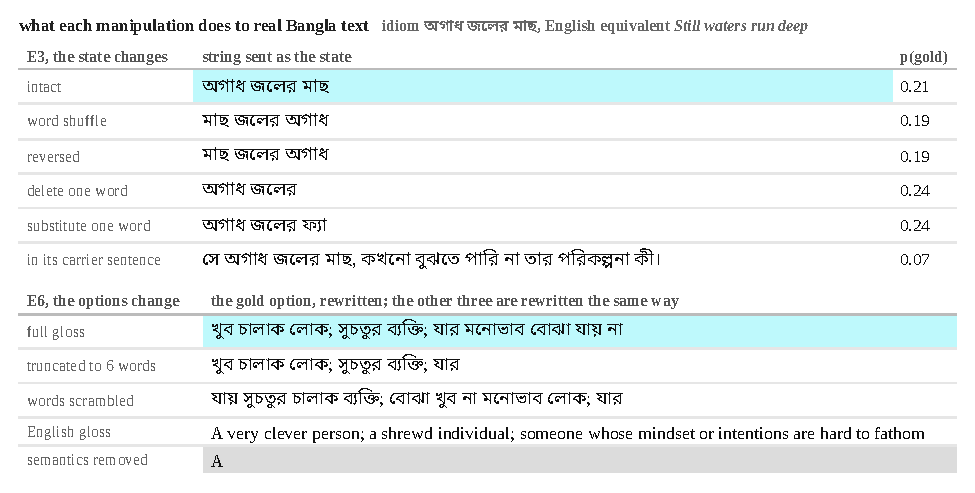
\includegraphics[width=\linewidth]{figures/fig_bn_manipulations.pdf}
% \caption{What the interventions do to real Bangla text, for the idiom
% \emph{agadh joler machh} (\emph{still waters run deep}, literally ``a fish of
% deep water''). \emph{Top:} the six E3 states, which are the exact strings logged
% during the run, with the probability the model gave the gold gloss. Shuffling and
% reversing a non-compositional expression leaves that probability essentially
% unchanged, and only the carrier sentence moves it. \emph{Bottom:} the five E6
% option forms, applied here to the gold option; the other three options are
% rewritten the same way. Truncation and word-scrambling preserve the lexical
% content that the scoring appears to depend on, while the last row removes it
% entirely and is the control of \S\ref{sec:nosignal}.}
% \label{fig:bnmanip}
% \end{figure*}



\begin{table*}[t]
\centering
\small
\renewcommand{\arraystretch}{1.15}

\begin{tabularx}{\textwidth}{
    @{}
    >{\raggedright\arraybackslash}p{2.05cm}
    >{\raggedright\arraybackslash}X
    >{\centering\arraybackslash}p{1.15cm}
    @{}
}
\toprule

\textbf{manipulation}
&
\textbf{string sent to the model}
&
\textbf{$p(\text{gold})$}
\\
\midrule

\multicolumn{3}{@{}l}{
    \textbf{E3: the state changes}
    \quad
    \textit{idiom: \bangla{অগাধ জলের মাছ}
    (\emph{Still waters run deep})}
}
\\[-1pt]

\textit{intact}
&
\cellcolor{fLaya}\bangla{অগাধ জলের মাছ}
&
\textbf{0.21}
\\

\textit{word shuffle}
&
\bangla{মাছ জলের অগাধ}
&
\textbf{0.19}
\\

\textit{reversed}
&
\bangla{মাছ জলের অগাধ}
&
\textbf{0.19}
\\

\textit{delete one word}
&
\bangla{অগাধ জলের}
&
\textbf{0.24}
\\

\textit{substitute one word}
&
\bangla{অগাধ জলের ফ্যা}
&
\textbf{0.24}
\\

\textit{in its carrier sentence}
&
\bangla{সে অগাধ জলের মাছ, কখনো বুঝতে পারি না তার পরিকল্পনা কী।}
&
\textbf{0.07}
\\[4pt]

\midrule

\multicolumn{3}{@{}l}{
    \textbf{E6: the options change}
    \quad
    \textit{gold option rewritten; the other three are rewritten identically}
}
\\[-1pt]

\textit{full gloss}
&
\cellcolor{fLaya}\bangla{খুব চালাক লোক; সুচতুর ব্যক্তি; যার মনোভাব বোঝা যায় না}
&
\\

\textit{truncated to 6 words}
&
\bangla{খুব চালাক লোক; সুচতুর ব্যক্তি; যার}
&
\\

\textit{words scrambled}
&
\bangla{যার সুচতুর চালাক ব্যক্তি; বোঝা খুব না মনোভাব লোক; যার}
&
\\

\textit{English gloss}
&
A very clever person; a shrewd individual; someone whose mindset or intentions are hard to fathom
&
\\

\textit{semantics removed}
&
\cellcolor{fGrey}\texttt{A}
&
\\

\bottomrule
\end{tabularx}

\caption{\textbf{What the interventions do to real Bangla text.}
The table shows the exact strings used for the idiom
\bangla{অগাধ জলের মাছ} (\emph{still waters run deep}, literally
``a fish of deep water''). \emph{E3} changes the state supplied to the
model; the reported probabilities are those assigned to the gold
figurative gloss. Shuffling and reversing the non-compositional
expression leave the probability essentially unchanged, whereas the
carrier sentence changes it. \emph{E6} changes the option text while
holding its role fixed; the five rows show increasingly reduced or
rearranged lexical content, ending with the semantics-free control.
The other three options undergo the same transformation as the gold
option.}

\label{tab:bnmanip}
\end{table*}




\section{Output distributions}
\label{app:dists}

The three arms do not merely differ in accuracy; they place their probability
mass very differently, and the shape of that mass is what makes the confidence
results of \S\ref{sec:confidence} possible. Table~\ref{tab:dist} summarises the
returned vectors.

\begin{table}[t]
\centering\small
\renewcommand{\arraystretch}{1.12}
\begin{tabularx}{\columnwidth}{@{}ll*{4}{>{\centering\arraybackslash}X}@{}}
\toprule
& & \textbf{Mean} & \textbf{Med.} & $\mathbf{>}\textbf{.95}$ & \textbf{Ent.} \\
\midrule
\multirow{2}{*}{Laya} &
\Drand & 0.438 & 0.408 & 0.001 & 0.892 \\
& \Dlit & 0.536 & 0.479 & 0.039 & 0.778 \\
\multirow{2}{*}{Lod} &
\Drand & 0.447 & 0.391 & 0.002 & 0.881 \\
& \Dlit & 0.745 & 0.819 & 0.171 & 0.497 \\
\multirow{2}{*}{Jev} &
\Drand & 0.967 & 1.000 & 0.852 & 0.068 \\
& \Dlit & 0.931 & 0.990 & 0.708 & 0.131 \\
\bottomrule
\end{tabularx}
\caption{Distribution of the returned maximum probability, and normalised
entropy of the full vector ($1=$ uniform). The literal-bearing family makes
both open arms \emph{sharper}, not flatter: Lod-lille's mean peak rises from
$0.447$ to $0.745$ and the share of near-deterministic answers from $0.002$ to
$0.171$, while its accuracy falls from $0.484$ to $0.066$. The model is not
confused by the literal gloss; it is convinced by it.}
\label{tab:dist}
\end{table}

That last point is worth stating separately, because it is the mechanism behind
the inverted reliability curves. A model that found the literal option merely
distracting would spread mass and lose accuracy together. Both open arms do the
opposite: adding the literal gloss \emph{concentrates} the distribution onto it.
On 24 items Laya-ml returns $p = 1.000$ on the literal gloss and $p = 0.000$ on
the gold.

\paragraph{Worked examples.} Table~\ref{tab:examples} gives four of them. The
idioms are transliterated because the toolchain cannot set Bengali script; the
released data carries the original strings.

\begin{table}[h]
\centering\small
\setlength{\tabcolsep}{3pt}
\begin{tabular}{llll}
\toprule
\textbf{Idiom} & \textbf{Literal} & \textbf{Figurative (gold)} & $p_{\text{lit}}$ \\
\midrule
\neu{tel} & \neu{oil} & \neu{arrogance} & \neu{1.000} \\
chamcha & spoon & sycophant & 1.000 \\
\neu{til} & \neu{sesame seed} & \neu{a tiny amount} & \neu{1.000} \\
charpaya & four-legged & rope cot & 1.000 \\
\bottomrule
\end{tabular}
\caption{Laya-ml under \Dlit. In each case the expert literal gloss and the
expert figurative gloss are both in the option list, and the model places all of
its mass on the literal reading. These are not hard or obscure idioms; three of
the four are single words in everyday use.}
\label{tab:examples}
\end{table}

% \begin{figure*}[t]
% \centering
% 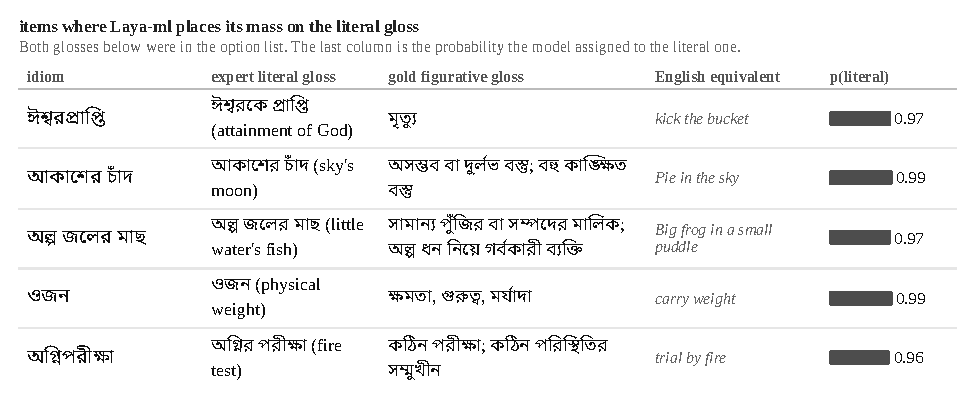
\includegraphics[width=\linewidth]{figures/fig_bn_examples.pdf}
% \caption{Five items on which Laya-ml assigns almost all of its probability to
% the idiom's own literal gloss, shown in Bengali with the English equivalent the
% annotators recorded. These are not obscure expressions:
% \emph{ishwarprapti} is the Bangla \emph{kick the bucket} and is read as
% ``attainment of God'', \emph{akasher chand} is \emph{pie in the sky} and is read
% as ``the moon of the sky''. Both glosses were present in the option list, and
% the right-hand column is the mass placed on the literal one.}
% \label{fig:bnexamples}
% \end{figure*}



\begin{table*}[t]
\centering
\small
\renewcommand{\arraystretch}{1.15}

\begin{tabularx}{\textwidth}{
    @{}
    >{\raggedright\arraybackslash}p{2.15cm}
    >{\raggedright\arraybackslash}p{3.0cm}
    >{\raggedright\arraybackslash}X
    >{\raggedright\arraybackslash}p{2.55cm}
    >{\centering\arraybackslash}p{1.35cm}
    @{}
}
\toprule

\textbf{idiom}
&
\textbf{expert literal gloss}
&
\textbf{gold figurative gloss}
&
\textbf{English equivalent}
&
\textbf{$p(\text{literal})$}
\\
\midrule

\bangla{ঈশ্বরপ্রাপ্তি}
&
\bangla{ঈশ্বরকে অধিগ্রহণ}
\newline
\emph{(attainment of God)}
&
\bangla{মৃত্যু}
\newline
\emph{(death)}
&
\emph{kick the bucket}
&
\cellcolor{fLaya}\textbf{0.97}
\\

\bangla{আকাশের চাঁদ}
&
\bangla{আকাশের চাঁদ}
\newline
\emph{(sky's moon)}
&
\bangla{অজন্তর বা দুর্লভ বস্তু; বহ কল্পিত বস্তু}
\newline
\emph{(an unattainable or rare object; an imagined object)}
&
\emph{pie in the sky}
&
\cellcolor{fLaya}\textbf{0.99}
\\

\bangla{অল্প জলের মাছ}
&
\bangla{অল্প জলের মাছ}
\newline
\emph{(little water's fish)}
&
\bangla{সামান্য পুঁজির বা সম্পদের মালিক; অল্প ধন নিয়ে দরিদ্র ব্যক্তি}
\newline
\emph{(a person with limited capital or resources; a poor person with little wealth)}
&
\emph{big frog in a small puddle}
&
\cellcolor{fLaya}\textbf{0.97}
\\

\bangla{ওজন}
&
\bangla{ওজন}
\newline
\emph{(physical weight)}
&
\bangla{ক্ষমতা, গুরুত্ব, মর্যাদা}
\newline
\emph{(power, importance, status)}
&
\emph{carry weight}
&
\cellcolor{fLaya}\textbf{0.99}
\\

\bangla{অগ্নিপরীক্ষা}
&
\bangla{আগুনের পরীক্ষা}
\newline
\emph{(fire test)}
&
\bangla{কঠিন পরীক্ষা; কঠিন পরিস্থিতির সম্মুখীন}
\newline
\emph{(a difficult test; facing a difficult situation)}
&
\emph{trial by fire}
&
\cellcolor{fLaya}\textbf{0.96}
\\

\bottomrule
\end{tabularx}

\caption{\textbf{Items where Laya-ml places almost all probability on the literal gloss.}
Each item contains the Bangla idiom, the expert-provided literal gloss,
the gold figurative gloss, and the English equivalent recorded by the
annotators. English translations in parentheses are provided for
readability; the underlying Bangla strings are the original dataset
content. Both literal and figurative glosses were present in the option
list. The rightmost column reports the probability assigned to the
literal gloss. These are not obscure expressions: \emph{ishwarprapti}
corresponds to \emph{kick the bucket} and is read literally as
``attainment of God,'' while \emph{akasher chand} corresponds to
\emph{pie in the sky} and is read literally as ``the moon of the sky.''}

\label{tab:bnexamples}
\end{table*}


\section{The capture matrix}
\label{app:matrix}

Table~\ref{tab:matrix} gives the six cells of \S\ref{sec:capture} with the
accuracy column alongside \LAR. All cells are $n = 3{,}265$ and were built by
one function from seed 21000; 95\% bootstrap intervals on \LAR{} are
$[.716,.746]$, $[.363,.397]$, $[.909,.928]$, $[.227,.256]$, $[.288,.319]$ and
$[.040,.055]$ reading down the table. The paired within-model language effect
on capture is $+0.352$ for Laya-ml, $+0.677$ for Lod-lille and $+0.256$ for
Jev-1.13, all McNemar $p < 10^{-100}$. Jev-1.13's English cell reproduces the
value reported from the original run, $0.0472$, which is why we treat the two
constructions as measuring the same thing.

\begin{table}[t]
\centering\small
\renewcommand{\arraystretch}{1.12}
\begin{tabularx}{\columnwidth}{@{}l>{\centering\arraybackslash}X>{\centering\arraybackslash}X>{\centering\arraybackslash}X>{\centering\arraybackslash}X@{}}
\toprule
& \multicolumn{2}{c}{\textbf{Bangla}} & \multicolumn{2}{c}{\textbf{English}} \\
\cmidrule(lr){2-3}\cmidrule(lr){4-5}
& \textbf{acc} & \textbf{\LAR} & \textbf{acc} & \textbf{\LAR} \\
\midrule
Laya-ml  & 0.127 & \textbf{0.731} & 0.417 & 0.379 \\
Lod-lille & 0.044 & \textbf{0.918} & 0.684 & 0.241 \\
Jev-1.13  & 0.536 & 0.304 & 0.926 & 0.047 \\
\bottomrule
\end{tabularx}
\caption{The literal condition as a model $\times$ language matrix, all six
cells measured on the same 3{,}265 items with one construction and one seed
($n=3{,}265$ per cell; 95\% CIs in Appendix~\ref{app:matrix}). Bold marks the
highest \LAR{} per language. Every arm is far more captured in Bangla than in
English, and the Bangla ordering does not follow capability: Jev-1.13 is the
most accurate and the least captured, while Lod-lille is more accurate than
Laya-ml and more captured.}
\label{tab:matrix}
\end{table}


% \begin{figure}[h]
% \centering
% 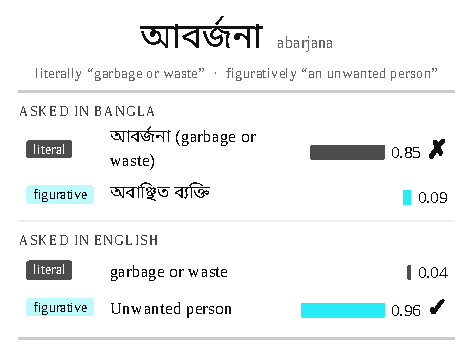
\includegraphics[width=\columnwidth]{figures/fig_bn_teaser.pdf}
% \caption{The same contrast on a second item, with the returned probabilities.
% \emph{Abarjana} means an unwanted person; its words mean garbage. Jev-1.13 is
% asked the identical question with the same four options in both languages: in
% Bangla it puts $0.85$ on the literal reading and $0.09$ on the gold, in English
% $0.96$ on the gold. Colour marks the option's role, not the model. This is
% Figure~\ref{fig:teaser}'s claim with the numbers attached.}
% \label{fig:bnteaser}
% \end{figure}




% \begin{figure}[t]
% \centering

% \begin{tikzpicture}[
%     x=1cm,
%     y=1cm,
%     line cap=round,
%     line join=round
% ]

% \definecolor{figCyan}{HTML}{27EBF5}
% \definecolor{figCyanLight}{HTML}{BEF9FC}
% \definecolor{figGray}{HTML}{4D4D4D}
% \definecolor{figRule}{HTML}{D0D0D0}

% % ─────────────────────────────────────────────────────────────────────
% % Header
% % ─────────────────────────────────────────────────────────────────────

% \node[
%     anchor=north,
%     font=\fontsize{20}{22}\selectfont
% ] at (0,0)
% {\bangla{আবর্জনা}};

% \node[
%     anchor=west,
%     font=\scriptsize\itshape,
%     text=gray
% ] at (1.25,-0.05)
% {abarjana};

% \node[
%     anchor=north,
%     font=\scriptsize,
%     text=gray
% ] at (0,-0.72)
% {literally ``garbage or waste''};

% \node[
%     anchor=north,
%     font=\scriptsize,
%     text=gray
% ] at (0,-1.02)
% {figuratively ``an unwanted person''};

% \draw[
%     figRule,
%     line width=0.5pt
% ] (-3.65,-1.32) -- (3.65,-1.32);

% % ─────────────────────────────────────────────────────────────────────
% % ASKED IN BANGLA
% % ─────────────────────────────────────────────────────────────────────

% \node[
%     anchor=west,
%     font=\bfseries\scriptsize,
%     text=figGray
% ] at (-3.55,-1.62)
% {ASKED IN BANGLA};

% % Literal label
% \node[
%     anchor=west,
%     rounded corners=1.5pt,
%     fill=figGray,
%     text=white,
%     inner xsep=4pt,
%     inner ysep=2pt,
%     font=\fontsize{6.5}{7}\selectfont
% ] at (-3.50,-2.08)
% {literal};

% % Figurative label
% \node[
%     anchor=west,
%     rounded corners=1.5pt,
%     fill=figCyanLight,
%     text=black,
%     inner xsep=4pt,
%     inner ysep=2pt,
%     font=\fontsize{6.5}{7}\selectfont
% ] at (-3.50,-2.78)
% {figurative};

% % Bangla options
% \node[
%     anchor=west,
%     font=\small
% ] at (-2.25,-2.08)
% {\bangla{আবর্জনা} (garbage or waste)};

% \node[
%     anchor=west,
%     font=\small
% ] at (-2.25,-2.78)
% {\bangla{অবাঞ্ছিত ব্যক্তি}};

% % Probability bars
% \draw[
%     figGray,
%     line width=4pt
% ] (0.35,-2.08) -- (2.65,-2.08);

% \node[
%     anchor=west,
%     font=\small
% ] at (2.85,-2.08)
% {0.85};

% \node[
%     anchor=west,
%     font=\bfseries\small
% ] at (3.35,-2.08)
% {\texttimes};

% \draw[
%     figCyan,
%     line width=4pt
% ] (0.35,-2.78) -- (0.59,-2.78);

% \node[
%     anchor=west,
%     font=\small
% ] at (2.85,-2.78)
% {0.09};

% % ─────────────────────────────────────────────────────────────────────
% % Separator
% % ─────────────────────────────────────────────────────────────────────

% \draw[
%     figRule,
%     line width=0.4pt
% ] (-3.50,-3.30) -- (3.50,-3.30);

% % ─────────────────────────────────────────────────────────────────────
% % ASKED IN ENGLISH
% % ─────────────────────────────────────────────────────────────────────

% \node[
%     anchor=west,
%     font=\bfseries\scriptsize,
%     text=figGray
% ] at (-3.55,-3.62)
% {ASKED IN ENGLISH};

% % Literal label
% \node[
%     anchor=west,
%     rounded corners=1.5pt,
%     fill=figGray,
%     text=white,
%     inner xsep=4pt,
%     inner ysep=2pt,
%     font=\fontsize{6.5}{7}\selectfont
% ] at (-3.50,-4.08)
% {literal};

% % Figurative label
% \node[
%     anchor=west,
%     rounded corners=1.5pt,
%     fill=figCyanLight,
%     text=black,
%     inner xsep=4pt,
%     inner ysep=2pt,
%     font=\fontsize{6.5}{7}\selectfont
% ] at (-3.50,-4.78)
% {figurative};

% % English options
% \node[
%     anchor=west,
%     font=\small
% ] at (-2.25,-4.08)
% {garbage or waste};

% \node[
%     anchor=west,
%     font=\small
% ] at (-2.25,-4.78)
% {Unwanted person};

% % Probability bars
% \draw[
%     figGray,
%     line width=4pt
% ] (0.35,-4.08) -- (0.46,-4.08);

% \node[
%     anchor=west,
%     font=\small
% ] at (2.85,-4.08)
% {0.04};

% \draw[
%     figCyan,
%     line width=4pt
% ] (0.35,-4.78) -- (2.95,-4.78);

% \node[
%     anchor=west,
%     font=\small
% ] at (2.85,-4.78)
% {0.96};

% \node[
%     anchor=west,
%     font=\bfseries\small
% ] at (3.35,-4.78)
% {\checkmark};

% % ─────────────────────────────────────────────────────────────────────
% % Bottom rule
% % ─────────────────────────────────────────────────────────────────────

% \draw[
%     figRule,
%     line width=0.5pt
% ] (-3.65,-5.30) -- (3.65,-5.30);

% \end{tikzpicture}

% \caption{\textbf{The same contrast on a second item, with the returned
% probabilities.}
% The Bangla idiom \bangla{আবর্জনা} (\emph{abarjana}) means ``an unwanted
% person'' figuratively, although its words mean ``garbage or waste''
% literally. Jev-1.13 is asked the identical question with the same four
% options in both languages: in Bangla it places $0.85$ on the literal
% reading and $0.09$ on the figurative gloss, whereas in English it places
% $0.96$ on the figurative gloss. Color marks the option's role, not the
% model.}

% \label{fig:bncontrast}
% \end{figure}








\section{How the two language cells were built}
\label{app:construction}

The capture matrix is the result we lean on hardest, so this appendix states
exactly how its two language cells were constructed, lists every asymmetry
between them that we could find, and reports the one test of the largest
asymmetry that the existing outputs permit.

\paragraph{Where the glosses come from.} Neither literal gloss is a translation
produced by us or by a machine. The corpus annotates one field per idiom,
\texttt{literal\_meaning}, written in Bangla with an English parenthetical
alongside it, so a single expert-authored field carries both readings. The Bangla
cell uses that field as written. The English cell uses the parenthetical alone,
recovered by a regular expression that accepts a parenthesised span only if it
contains at least three ASCII letters and is at least $60\%$ ASCII by character,
which excludes Bangla asides and bare numerals. Of $8{,}876$ items, $3{,}391$
carry such a parenthetical, $3{,}352$ of those also carry an English equivalent
idiom, and $3{,}265$ survive a final cut requiring the English literal gloss to be
lexically distinct from the English gold gloss (Jaccard $< 0.34$). That pool of
$3{,}265$ is the matrix. The provenance matters because a machine-translated
English gloss would make the English cell a measurement of the translator; an
annotator-written one does not.

\paragraph{The four asymmetries.} We can state these precisely, which is better
than asserting the cells are matched.

\emph{(i) The state differs in kind.} The Bangla state is the idiom itself. The
English state is the annotator's nearest English idiom, taken from the
\texttt{similar\_in\_english} field, not a translation of the Bangla one. The
cells are therefore paired entries, and we use that phrase in the paper rather
than ``identical items''.

\emph{(ii) The Bangla literal option is bilingual.} Because the Bangla cell uses
the annotated field as written, and pool membership requires that field to contain
an English parenthetical, every one of the $3{,}265$ Bangla literal options
contains its own English gloss inside it. It averages $44$ characters against $24$
for the English literal option. We did not strip the parenthetical, because doing
so would have meant presenting the open arms a string the corpus does not
contain; the cost is that the Bangla literal distractor is longer and partly in
the other script.

\emph{(iii) The distinctness cut applies to one side only.} The Jaccard
$< 0.34$ filter between gold and literal gloss was applied in English and not in
Bangla. Measured after the fact, the filter turns out not to bind: mean gold-versus-literal
Jaccard is $0.029$ in Bangla against $0.052$ in English, so the
Bangla side is the more separated of the two and would have passed the cut almost
everywhere. This asymmetry is procedural rather than consequential.

\emph{(iv) The literal gloss echoes the state more often in Bangla.} This is the
one that could plausibly manufacture the result. The Bangla literal gloss shares at
least one content word with the Bangla idiom on $56.2\%$ of pool items; the English
literal gloss shares one with the English equivalent idiom on $25.1\%$. A model
doing order-free lexical matching on the option side, which
\S\ref{sec:bagofwords} shows all three partly are, has a surface hook into the
Bangla literal option that it lacks in English.

\paragraph{Testing asymmetry (iv).} The existing per-item outputs are enough to
test it without running anything new. Split the pool on whether the Bangla literal
gloss shares a content word with the idiom and read \LAR{} in each stratum
(Table~\ref{tab:construction}, upper block). If the hook were driving capture, the
overlap stratum would be far more captured in every arm. It is not: the effect is
$+0.026$ for Laya-ml, $+0.130$ for Lod-lille and $-0.129$ for Jev-1.13. The sign
is not even consistent across arms, and on the commercial arm the hook is
associated with \emph{less} capture, which is the opposite of the predicted
direction.

The sharper test restricts both language cells to the $1{,}429$ items where the
hook is absent and re-reads the gap there (lower block). It barely moves: $+0.358$,
$+0.610$ and $+0.310$, against headline gaps of $+0.352$, $+0.677$ and $+0.256$.
For two of the three arms the gap is slightly \emph{larger} once the hook is
removed. We read this as showing that asymmetry (iv) does not account for the
Bangla--English difference, not as showing the cells are equivalent; a corpus
paired by translation rather than by annotator judgement would settle what we can
only bound here.

\begin{table}[t]
\centering\small
\renewcommand{\arraystretch}{1.12}
\begin{tabularx}{\columnwidth}{@{}>{\raggedright\arraybackslash}X>{\centering\arraybackslash}p{1.05cm}>{\centering\arraybackslash}p{1.05cm}>{\centering\arraybackslash}p{1.05cm}@{}}
\toprule
& \textbf{Laya} & \textbf{Lod} & \textbf{Jev} \\
\midrule
\multicolumn{4}{@{}l}{\emph{Bangla \LAR{} by surface hook}} \\
hook absent ($n=1429$)  & 0.716 & 0.845 & 0.376 \\
hook present ($n=1836$) & 0.742 & 0.975 & 0.247 \\
difference              & $+0.026$ & $+0.130$ & $-0.129$ \\
\addlinespace
\multicolumn{4}{@{}l}{\emph{Capture gap, hook-absent items only}} \\
Bangla \LAR            & 0.716 & 0.845 & 0.376 \\
English \LAR           & 0.358 & 0.236 & 0.066 \\
gap                    & $+0.358$ & $+0.610$ & $+0.310$ \\
\addlinespace
headline gap (all pool) & $+0.352$ & $+0.677$ & $+0.256$ \\
\bottomrule
\end{tabularx}
\caption{\textbf{The construction asymmetry does not carry the result.}
\swL Laya-ml, \swD Lod-lille, \swJ Jev-1.13. ``Hook'' means the Bangla literal
gloss shares at least one content word with the idiom, which is the asymmetry
most likely to inflate Bangla capture. Upper block: capture is not reliably higher
when the hook is present, and on the commercial arm it is lower. Lower block:
restricting both language cells to hook-absent items leaves the capture gap
essentially unchanged, and larger for two of three arms. The script is released
with the per-item outputs.}
\label{tab:construction}
\end{table}

\paragraph{What this appendix does not establish.} It tests one asymmetry, the one
we could operationalise from recorded outputs. Asymmetries (i) and (ii) are
structural and cannot be tested without new data: we cannot ask what the arms
would do on a Bangla literal option with its parenthetical stripped, or on an
English state that is a literal translation rather than an idiomatic equivalent,
without running those conditions. We flag them in Limitations rather than
dismissing them.

\section{Cross-lingual arms}
\label{app:crossling}

Figure~\ref{fig:crosslingual} plots the E4 conditions discussed in
\S\ref{sec:crosslingual}.

\begin{figure*}[!tbp]
\centering
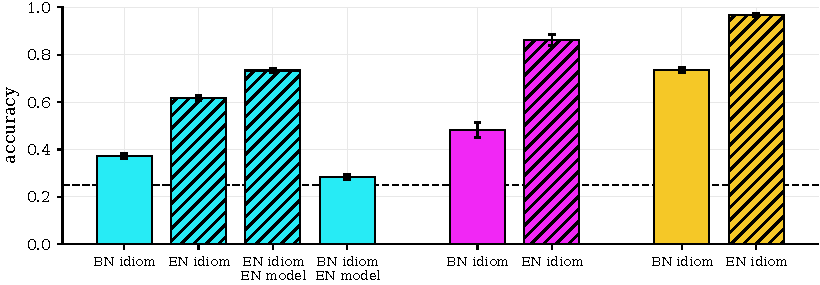
\includegraphics[width=0.74\linewidth]{figures/fig10_crosslingual.pdf}
\caption{Accuracy by task language, grouped by model: \swL Laya-ml (four bars),
\swD Lod-lille, \swJ Jev-1.13. \textbf{Solid} bars are Bangla input,
\textbf{hatched} bars English; Laya-ml's third and fourth
bars use the English-only checkpoint, the fourth being the control. Error bars
95\% bootstrap CIs, dashed line chance. Every model gains 20--45 points from the
same idiom presented in English.}
\label{fig:crosslingual}
\end{figure*}

\section{The matched three-way condition}
\label{app:threeway}

Figure~\ref{fig:threeway} plots Table~\ref{tab:threeway}, the one condition
that is identical across all three arms.

\begin{figure}[t]
\centering
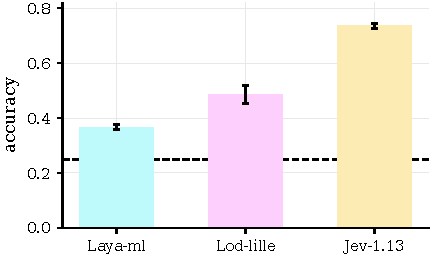
\includegraphics[width=\columnwidth]{figures/fig3_three_way_bangla.pdf}
\caption{The matched three-way comparison. Bars left to right: \swL Laya-ml,
\swD Lod-lille, \swJ Jev-1.13. Black dashed line is chance, error bars 95\%
bootstrap CIs. This capability
ordering is the baseline against which the calibration failures in
\S\ref{sec:confidence}--\S\ref{sec:nosignal} should be read.}
\label{fig:threeway}
\end{figure}

\section{Unit integrity}
\label{app:unit}

Figure~\ref{fig:unit} plots the E3 perturbations described in \S\ref{sec:unit}. The options are byte-identical across all six variants, so the only difference reaching the model is the state string.

\begin{figure*}[!tbp]
\centering
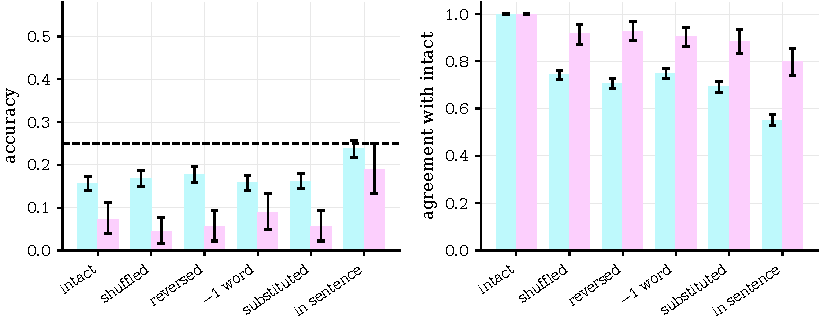
\includegraphics[width=0.80\linewidth]{figures/fig9_unit_integrity.pdf}
\caption{Unit integrity: the idiom is perturbed, the options held fixed.
\swL Laya-ml, \swD Lod-lille; error bars 95\% bootstrap
CIs, dashed line chance (left panel). \emph{Left:} accuracy. \emph{Right:}
agreement with the answer on the intact idiom. Scrambling and reversing a
non-compositional expression does not meaningfully hurt either model, which is
the
bag-of-words signature.}
\label{fig:unit}
\end{figure*}

\section{Surface invariance}
\label{app:surface}

The corpus ships alternative surface forms certified by annotators as
meaning-preserving. A model reading meaning should be invariant across such a
pair. Laya-ml agrees with itself on $0.657$ of 3{,}143 pairs (2{,}423 items) and
Lod-lille on $0.677$ of 310 pairs (234 items): about a third of the time, a
meaning-preserving rewrite changes the answer. Mean Jensen--Shannon divergence
between the two probability vectors is $0.039$ and $0.085$.

\section{Subset representativeness}
\label{app:subset}

Lod-lille ran a fixed 10\% random subset. Table~\ref{tab:subset} compares
Laya-ml's accuracy on those same 888 items against its own full 8{,}876.

\begin{table}[t]
\centering\small
\renewcommand{\arraystretch}{1.12}
\begin{tabularx}{\columnwidth}{@{}>{\raggedright\arraybackslash}X>{\centering\arraybackslash}p{1.35cm}>{\centering\arraybackslash}p{1.35cm}>{\centering\arraybackslash}p{1.15cm}@{}}
\toprule
\textbf{Family} & \textbf{Full} & \textbf{Subset} & \textbf{Drift} \\
\midrule
\Drand & 0.367 & 0.351 & $-0.016$ \\
\Dsurf & 0.338 & 0.339 & $+0.001$ \\
\Dsem  & 0.333 & 0.325 & $-0.007$ \\
\Dlit  & 0.151 & 0.136 & $-0.015$ \\
\Dhard & 0.144 & 0.149 & $+0.004$ \\
\bottomrule
\end{tabularx}
\caption{Laya-ml on the 10\% subset against its own full set. Maximum drift
is $0.016$. Two of five subset estimates fall marginally outside the full-set
bootstrap CI, which is expected at $n=888$ and changes no sign or ordering.
The full-set figures are therefore reported as the precise estimates.}
\label{tab:subset}
\end{table}

\section{Full option ablation}
\label{app:options}

Table~\ref{tab:options} gives the numbers behind Figure~\ref{fig:options}.

\begin{table}[t]
\centering\small
\renewcommand{\arraystretch}{1.12}
\begin{tabularx}{\columnwidth}{@{}>{\raggedright\arraybackslash}X>{\centering\arraybackslash}p{1.05cm}>{\centering\arraybackslash}p{1.05cm}>{\centering\arraybackslash}p{1.05cm}@{}}
\toprule
\textbf{Option text} & \textbf{Laya} & \textbf{Lod} & \textbf{Jev} \\
\midrule
full gloss   & 0.365 & 0.492 & 0.970 \\
truncated    & 0.361 & 0.468 & 0.958 \\
scrambled    & 0.357 & 0.479 & 0.974 \\
other lang.  & 0.347 & 0.398 & 0.963 \\
no semantics & 0.256 & 0.233 & 0.254 \\
\bottomrule
\end{tabularx}
\caption{\textbf{Option-side ablation.}
The semantics-free row removes meaningful option content and yields
near-chance accuracy in all three arms. Jev-1.13's column is English.}
\label{tab:options}
\end{table}

\begin{figure*}[t]
\centering
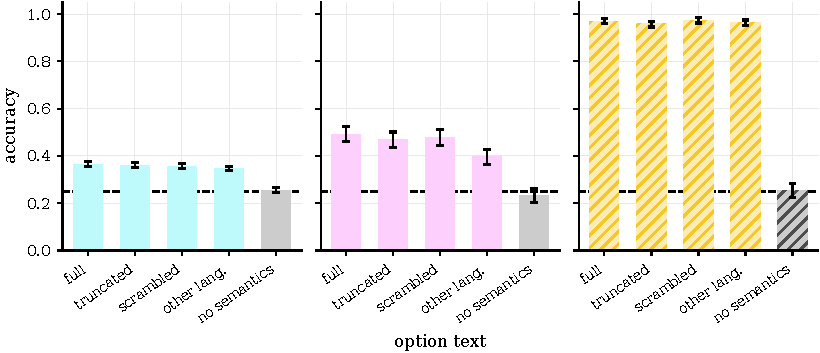
\includegraphics[width=0.90\linewidth]{figures/fig8_option_ablation.pdf}
\caption{Option-side ablation. Panels left to right: \swL Laya-ml, \swD Lod-lille,
\swJ Jev-1.13. In each panel the fifth, \swG bar is the semantics-free control
of \S\ref{sec:nosignal}; the whole Jev-1.13 panel is
hatched because its task is in \textbf{English}. Error bars are 95\% bootstrap
CIs and the black dashed line is chance. Truncating and word-scrambling the
option text cost almost nothing in any of the three models.}
\label{fig:options}
\end{figure*}

\section{Order sensitivity and position bias}
\label{app:position}

This appendix reports the per-slot selection shares behind \S\ref{sec:order},
then sets out the permutation audit that establishes the residual instability of
the independent-option scorer is real rather than an artifact of our harness.

\paragraph{What is held fixed.} Each item here is one idiom with one fixed set of
four option texts. We present that same set 24 times, once per permutation, and
change nothing else: the instruction string, the state, $k$, the decoding
configuration and the option texts themselves are byte-identical across the 24
calls, and no call is retried. The only quantity that varies is which slot each
option occupies. Anything that moves across the 24 calls is therefore
attributable to order, which is what makes this the cleanest of our seven
interventions.

\paragraph{Recovering option identity.} The harness records, per call, the
permutation as a four-digit string in which position $s$ holds the index, in the
canonical option list, of the option displayed in slot $s$. A chosen slot must be
mapped back through that permutation before it can be compared across calls.
Counting distinct slot \emph{letters} instead inflates instability to near unity
for any scorer, because a letter necessarily changes whenever the same gloss is
moved, and we report this because an earlier draft of our own analysis made that
mistake. All numbers in the paper use the mapped gloss identity.

\paragraph{The permutation audit.} Table~\ref{tab:orderaudit} reports a quantity
that the summary measures in Table~\ref{tab:order} cannot: not whether the
\emph{answer} changes, but how far a \emph{single option's own score} travels as
that option is moved around the list. This is the quantity the independent-option
design makes a claim about. Scoring each option in its own forward pass should
make an option's score a function of the option and the state alone, so the
spread should sit at the level of floating-point accumulation noise, which for
\texttt{fp32} summation over sequences of this length is on the order of
$10^{-7}$. It does not. Lod-lille's median item has an option whose score moves
$4.0 \times 10^{-2}$, five orders of magnitude higher, and not one of its 299
items falls below $10^{-4}$. Two consequences follow. First, the $10.7\%$
answer-change rate in Table~\ref{tab:order} is not a tie-breaking artifact: ties
would require near-identical scores, and the scores are not near-identical.
Second, the documented guarantee is not one an evaluation can rely on, at least
in the configuration we were able to run.

\begin{table}[t]
\centering\small
\renewcommand{\arraystretch}{1.12}
\begin{tabularx}{\columnwidth}{@{}>{\raggedright\arraybackslash}X>{\centering\arraybackslash}p{1.05cm}>{\centering\arraybackslash}p{1.05cm}>{\centering\arraybackslash}p{1.05cm}@{}}
\toprule
& \textbf{Laya} & \textbf{Lod} & \textbf{Jev} \\
\midrule
items                       & 992   & 299   & 300   \\
median spread               & \textbf{0.495} & 0.040 & 0.070 \\
mean spread                 & \textbf{0.507} & 0.046 & 0.139 \\
95th pct.\ spread           & \textbf{0.772} & 0.105 & 0.480 \\
max spread                  & \textbf{0.928} & 0.245 & 0.820 \\
share $< 10^{-4}$           & 0.000 & 0.000 & \textbf{0.230} \\
answer changes              & \textbf{0.837} & 0.107 & 0.133 \\
\bottomrule
\end{tabularx}
\caption{\textbf{Permutation audit.} Per item, the largest distance a single
option's own score travels across the 24 orderings of its list, after mapping
each slot back to the option it displayed.
\swL Laya-ml, \swD Lod-lille, \swJ Jev-1.13. Bold marks the largest value in each
row. An order-independent scorer should sit at \texttt{fp32} noise, around
$10^{-7}$; the \emph{share} row gives the fraction of items at or below
$10^{-4}$, a threshold three orders of magnitude more permissive than that. Only
Jev-1.13 returns bit-identical distributions on any item, and then on fewer than
a quarter of them. The script that produces this table is released with the
per-item outputs.}
\label{tab:orderaudit}
\end{table}

\paragraph{The commercial arm.} Jev-1.13 makes no public invariance claim, and
its behaviour is the least like either open arm: it is the only arm that returns
bit-identical distributions on some items at all, on $23.0\%$ of them, yet its
mean spread ($0.139$) is three times Lod-lille's and its maximum ($0.820$)
approaches Laya-ml's. The distribution is bimodal rather than merely noisier,
which is what one would expect from a scorer that is close to deterministic on
easy items and switches regime on hard ones. We cannot test that reading without
weights, and we do not claim it.

\paragraph{Position bias.} Figure~\ref{fig:position} gives the per-slot selection
shares. Because the gold option is placed uniformly at random, the expectation
under no positional bias is exactly $0.25$ in every slot for every arm, so this
figure needs no baseline model: the distance from the dashed line \emph{is} the
bias. Laya-ml's profile is not the primacy gradient usually reported for prompted
generative scorers \citep{zheng2024robust}; it peaks on slot B at $37.2\%$
against $14.6\%$ for slot A, which is a $2.6\times$ accuracy swing from position
alone and is not a monotone function of position at all. We note the shape and
decline to explain it; with one model per scoring design, we have no way to
separate a property of the marker scheme from a property of this particular
backbone.

\begin{figure*}[t]
\centering
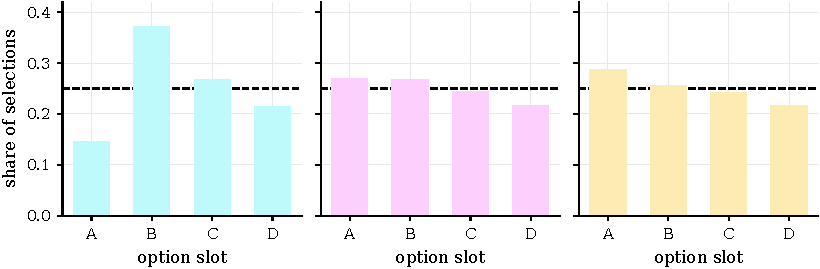
\includegraphics[width=0.90\linewidth]{figures/fig7_position_bias.pdf}
\caption{Share of selections falling on each option slot. Panels left to right:
\swL Laya-ml, \swD Lod-lille, \swJ Jev-1.13. The gold option is placed
uniformly at random, so the black dashed line at $0.25$ is the expectation under
no positional bias and any departure from it is bias. Laya-ml peaks on slot B,
taking it $37.2\%$ of the time against $14.6\%$ for slot A; the other two arms sit
close to the line throughout, with a mild and monotone preference for earlier
slots.}
\label{fig:position}
\end{figure*}

\begin{figure*}[t]
\centering
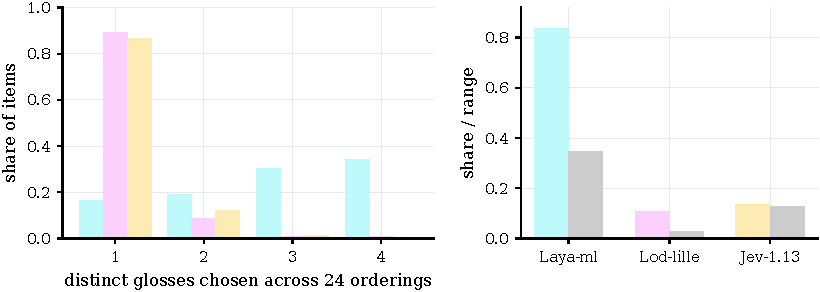
\includegraphics[width=0.90\linewidth]{figures/fig6_order_sensitivity.pdf}
\caption{Order sensitivity. \emph{Left:} how many distinct glosses each model
selects across the 24 orderings of one option set; within each group bars run \swL Laya-ml,
\swD Lod-lille, \swJ Jev-1.13, and a value of 1 means perfect stability.
\emph{Right:} per model, the coloured bar is the share of items whose chosen
gloss is unstable and the \swG bar is the mean within-item range of $p$(gold). Laya-ml is
unstable on 83.7\% of items with a mean $p$(gold) swing of $0.346$; the other two
are near-stable.}
\label{fig:order}
\end{figure*}

\section{Run record}
\label{app:repro}

\paragraph{Environment.} Python 3.13.15 throughout. The two open arms ran on one
Tesla T4 (15{,}360\,MiB): Laya-ml in \texttt{bf16} with \texttt{max\_len} 1024
at 27.2\,ms per call, Lod-lille in \texttt{fp32} at 86.1\,ms per call. The
commercial arm needs no accelerator and ran on CPU against
\texttt{typesafe/jev-1.13}.

\paragraph{Temperatures.} Laya-ml's run recorded
\texttt{temperature = [1.0, 1.0, 1.0]} with \texttt{temperature\_by\_options}
empty, so the per-bucket temperatures it ships were not applied and its ECE
figures are raw. Lod-lille ships \texttt{temperature: 1.0} by design, its
authors having reported that fitting hurt held-out calibration. Both open arms
are therefore untempered and comparable on that axis. The commercial arm's
internal calibration is not observable.

\paragraph{Seeds.} The Bangla arms use a per-experiment seed (E1 1000, E2 2000,
E3 3000, E4 4000, E6 6000, E7 7000) added to the item id, so each item's option
permutation is reproducible and identical across arms. The split seed is
20261001. The commercial arm uses a disjoint block seed set (order audit 17000,
literal 12000, ceiling 11000, Bengali control 14000, options 16000) because its
blocks ran in a different order; the permutation for a given item is still a
pure function of seed and id.

\paragraph{Call volume and cost.} The commercial arm issued 56{,}533 calls for
\$0.9348 at \$0.042 per million input tokens with output free. The blocks are
the order audit ($300 \times 24 = 7{,}200$), literal capture on the shared pool
($3{,}265 \times 3 = 9{,}795$), the English ceiling ($8{,}761 \times 3 =
26{,}283$), the Bengali control ($8{,}761$) and the option ablation ($873
\times 5 = 4{,}365$), which is 56{,}404 retained rows. The remaining 129 calls
are the endpoint probe and the response-contract checks made before each block.
Transient 429 and 5xx responses were retried with exponential backoff to a
30\,s ceiling; no call was dropped.

\paragraph{Statistics.} All intervals are 95\% percentile bootstrap over items,
2{,}000 resamples, fixed seed 0. ECE uses 15 equal-width bins. Paired
comparisons use McNemar's exact test via the binomial distribution. AURC is
reported against a random-gate baseline computed on the same items.

\paragraph{What is released.} The per-item outputs for every cell of every
experiment (one row per item per condition, carrying the full probability
vector, the predicted key, the gold key, the literal key and the gold position),
the five split manifests, the three run environment records quoted above, the
task configurations containing the verbatim instruction strings, the analysis
scripts that turn those outputs into every table in this paper, the figure
sources, and a CSV of the exact plotted values beside each figure.

\paragraph{Pairing.} Because the two open arms were reconstructed independently
from a written contract rather than from shared code, the released outputs admit
a direct check: on the 4{,}440 overlapping rows the gold key, gold position,
idiom string and literal-distractor key agree at $1.000$. That check is itself a
released artifact, and it is what licenses every paired test in the paper.

\paragraph{The matrix run.} The six cells of \S\ref{sec:capture} were run
afterwards as one job, with its own seed namespace (21000) so no option
permutation collides with the runs above. Every cell covers the same 3{,}265
items and is built by a single function; the two languages share one distractor
draw per item and are shuffled independently from the same generator. Laya-ml
ran both languages on the multilingual checkpoint, so only the language changes
and the checkpoint does not. Lod-lille ran the full pool rather than its earlier
10\% subset, which supersedes the thin 316-item in-pool estimate. The
commercial arm issued 6{,}531 calls for \$0.1152. Its English cell reproduces
the value from the original run to four decimal places ($0.0472$), which is the
check that the two constructions measure the same thing.

\paragraph{Known gaps.} E2 was not run on the commercial arm, because the
alternative surface forms exist only in Bangla and the arm's task is English.
The matrix covers the literal condition only; the other distractor families were
not run in both languages. The confidence and calibration results remain
two-arm, because the commercial arm's reliability was measured on its English
run.

\end{document}
